\documentclass[oneside, ngerman, toc=bibliography,bibliography=totoc,listof=entryprefix, open=right,numbers=noenddot,fontsize=12pt]{scrbook}

% für sabine 14pt setzen

\usepackage{ngerman}
\usepackage[ngerman]{babel}
%\usepackage[german]{hyphenat}
\sloppy 
\usepackage[none]{hyphenat}  % stelle die meist falsche silbentrennung ab

\usepackage[onehalfspacing]{setspace}

\usepackage[T1]{fontenc}
\usepackage[utf8]{inputenc}
\usepackage{cmap}
%\usepackage{bibgerm} % Verwendet deutsche Abkürzungen

\usepackage[a4paper, left= 3cm, right=2cm, top=2.5cm, bottom=2cm, includeheadfoot]{geometry}




\usepackage{booktabs} % Benutze booktabs, um korrekt gesetzte, SCHOENE Tabelle zu erzeugen http://www.math.utah.edu/tex-archive/macros/latex/contrib/booktabs/booktabs.pdf

\usepackage{longtable} % Für Tabellen, die länger als eine Seite sind. Der Seitenumbruch erfolgt dann automatisch. Bsp.: Glossar

\usepackage{times} % andere schrift

% jpeg png etc. erlauben
\usepackage{graphicx}
\usepackage{epsfig}
\usepackage{graphics}
%\usepackage{color}
\usepackage{xcolor} 
% Komfortableres Tabellen-Paket
\usepackage{tabularx}
\usepackage{tabu}
% Ermöglicht mehrere Bilder in einer floatenden Figure-Umgebung
%\usepackage{subfig}
%\usepackage{ulem}
%\usepackage{csquotes}



% Erlauben von urls
\usepackage{url}
\usepackage{hyperref}
\usepackage{letterspace}	% For extended line spacing on title page

%\usepackage[overload]{textcase}
% \usepackage{listings}
 
%python Pygments und -shell-escape
% \usepackage{minted}
\usepackage[framemethod=default]{mdframed}

\newcommand{\autor}{Jens Kapitza}
\newcommand{\titel}{SciServer -- Entwicklung einer Serversoftware zur Verwaltung von wissenschaftlichen Daten}
\newcommand{\ort}{Duisburg}
\newcommand{\einreichung}{20.10.2015}
\newcommand{\matrikelnr}{2242777}
\newcommand{\studiengang}{Angewandte Informatik}
\newcommand{\arbeit}{Masterarbeit}
\newcommand{\erstpruefer}{Prof.\ Jens Krüger}
\newcommand{\zweitpruefer}{Prof.\ Torben Weis}
\newcommand{\abschluss}{Master of Science (M. Sc.)}

% Klickbare Links innerhalb des PDFs
\hypersetup{ pdftitle={SciServer}, pdfauthor={\autor{}}, pdfsubject={\arbeit{}}, colorlinks=false, breaklinks=true }



% andere schrift beim zitieren
\AtBeginEnvironment{quote}{\setlength{\textwidth}{0.7\textwidth}\itshape\small}

\newcommand\chapmd[2]{\begin{mdframed}[%
		rightline=false,leftline=false,topline=false,bottomline=false,frametitlerule=false,
		userdefinedwidth=\textwidth,frametitlealignment=\flushright, %frametitlebackgroundcolor=gray!5,
		frametitlerulecolor=black,frametitle={\small #1}]
		\flushright{} \footnotesize{} #2
	\end{mdframed}}

% Style Minted
%\usemintedstyle{default}
%\newminted{java}{linenos=true, numbersep=5pt,fontsize=\footnotesize,texcl=true}
%\newminted{xml}{linenos=true,numbersep=5pt,fontsize=\footnotesize,texcl=true}
%\newminted{shell}{linenos=true,numbersep=5pt,fontsize=\footnotesize,texcl=true}

\usepackage[nonumberlist,nopostdot]{glossaries}
\makeglossaries
\usepackage[xindy]{imakeidx}
\makeindex



\usepackage{xparse}
\DeclareDocumentCommand{\newdualentry}{ O{} O{} m m m m } {
    \newglossaryentry{gls-#3}{name={#5},text={#5\glsadd{#3}}, description={#6},#1}
    
    \newacronym[see={[Glossary:]{gls-#3}},#2]{#3}{#4}{#5\glsadd{gls-#3}}
}

\begin{document}


\newdualentry{dms} % label
{DMS}            % abbreviation
{Datenmanagementsystem}  % long form
{System zum Verwalten von Dateien, in dem auch gesucht werden kann.} % description
 
\newdualentry{p2p} % label
{P2P}            % abbreviation
{Peer-to-Peer}  % long form
{Kommunikationsmodell, in dem jeder Teilnehmer mit jedem anderen reden kann.} % description
 
\newdualentry{nfs} % label
{NFS}            % abbreviation
{Network File System}  % long form
{Bei Linux gleichnamiger Dienst, generell ist ein Netzwerkdienst gemeint, welcher sein Dateisystem über einen Computer hinweg zur Verfügung stellt.} % description
 
\newdualentry{cifs} % label
{CIFS}            % abbreviation
{Common Internet File System}  % long form
{Netzwerk Kommunikationsprotokoll, unter Windows und durch Samba unter Linux bereitgestellter Dienst zum Datenaustausch zwischen Computern.} % description

\newdualentry{ads} % label
{ADS}            % abbreviation
{alternative data streams}  % long form
{Windows Funktion zur Datenspeicherung innerhalb einer Datei} % description
 
\newdualentry{rf} % label
{RF}            % abbreviation
{resource forks}  % long form
{Eine Technologie, die von Apple verwendet wurde, zur Datenspeicherung innerhalb einer Datei.} % description

\newdualentry{lvm} % label
{LVM}            % abbreviation
{Logical-Volume-Manager}  % long form
{Ein LVM, bietet einen virtuellen Zusammenschluss mehrerer Festplatten zu einem logischen Laufwerk. } % description



\newdualentry{rpc} % label
{RPC}            % abbreviation
{Remote Procedure Call}  % long form
{Aufruf einer fernen Prozedur} % description



\newdualentry{nat} % label
{NAT}            % abbreviation
{Network Address Translation}  % long form
{Verfahren zum Ersetzen der Adressinformationen in IP Datenpaketen} % description


\newdualentry{jms} % label
{JMS}            % abbreviation
{Java Message Service}  % long form
{Bibliothek zum Kommunizieren durch Nachrichtenaustausch. } % description
 
 \newdualentry{pae} % label
 {PAE}            % abbreviation
 {Physical Address Extension}  % long form
 {Erweiterung der Adressierung in 32 Bit Architektur} % description
 
 
\newdualentry{cdi} % label
{CDI}            % abbreviation
{Contexts and Dependency Injection}  % long form
{Aus Java EE, Möglichkeit zur Auflösung von Objektabhängigkeiten zur Laufzeit sowie Verwaltung von Lebenszyklen verwalteter Objekte innerhalb einer Anwendung.} % description

\newdualentry{jpa} % label
{JPA}            % abbreviation
{Java Persistence API}  % long form
{API in Java zur Verwendung einer Datenbank, diese API beinhaltet auch eine \acrshort{orm} Abbildung von Klassen auf Tabellen der Datenbank.} % description
 
\newdualentry{orm} % label
{ORM}            % abbreviation
{Object-Relational Mapping}  % long form
{Bidirektionale Abbildung der Spalteninformationen einer Datenbank in Eigenschaften eines Objektes.} % description

\newdualentry{tls} % label
{TLS}            % abbreviation
{Transport Layer Security}  % long form
{Verschlüsselung durch Zertifikate, häufige Verwendung bei HTTPS, SMTPS, FTPS. Sollte nicht mit SFTP verwechselt werden, welches ein anderes Verfahren nutzt (Schlagwort: SSH).} % description
 

\newdualentry{ide} % label
{IDE}            % abbreviation
{Integrierte Entwicklungsumgebung}  % long form
{Eine IDE erlaubt das einfachere Schreiben von Quellcode und unterstützt verschiedene Tools, die das Arbeiten z. B. mit Datenbanken vereinfachen.} % description




\newdualentry{ttl} % label
{TTL}            % abbreviation
{Time to live}  % long form
{Lebenszeit, z. B. für ein Verwerfen eines Paketes im Netzwerk.} % description


 
\newdualentry{fqdn} % label
{FQDN}            % abbreviation
{Fully Qualified Domain Name}  % long form
{Absoluter vollständiger Domainname eines Computers.} % description
  
 
 
 
 \newdualentry{stun} % label
 {STUN}            % abbreviation
 {Session Traversal Utilities for NAT}  % long form
 {Möglichkeit zum Erkennen der externen Verbindungsparameter sowie den \acrshort{nat} Firewall-Typen für anfragende Geräte.} % description
 
  
 
 \newdualentry{acc} % label
 {ACC}            % abbreviation
 {Application Client Container}  % long form
 {Spezielle Form eines Clients, der komplett vom Anwendungsserver abhängig ist.} % description
 
 \newdualentry{KEY} % label
 {ABBR}            % abbreviation
 {LONG}  % long form
 {DESC} % description
 
 
 
 

\author{\autor{}}
\title{\titel{}}
\date{\einreichung{}}


\frontmatter
\pagenumbering{Roman}

\begin{titlepage}
%\enlargethispage{2cm}

\includegraphics[width=6cm]{uni-logo.pdf}\\
\\[1cm] 
\vspace*{4cm}\noindent
\textls[70]{ \Large{\sf{\MakeTextUppercase{\arbeit{}}}}}\\
\huge{\sf{ \textbf{\titel{}}}}\\[1cm]
\textls[70]{\Large{\sf{von \autor{} (Matrikel-Nr.: \matrikelnr{})}}}%[6cm]

\vspace*{\fill}
\normalsize
\begin{center}
\begin{tabularx}{0.9\textwidth}{Xl}
      & Erstprüfer: \erstpruefer{}\\
      & Zweitprüfer: \zweitpruefer{}
\end{tabularx}
\end{center}

\vspace*{1cm}
Eine Abschlussarbeit im Studiengang \studiengang{}, vorgelegt der Abteilung Informatik und Angewandte Kognitionswissenschaft an der Universität Duisburg-Essen zur Erlangung des akademischen Grades \abschluss{}.
\end{titlepage}


\cleardoublepage
\vspace*{\fill}
\section*{Zusammenfassung}


Zeitgemäße Datenspeicherung erfordert ein einfaches und effizientes Suchen über die gespeicherten Daten. Da Weboberflächen immer beliebter werden, gerade durch die mobilen Endgeräte, wird im Rahmen dieser Masterarbeit ein Such- und Benachrichtigungssystem mit deren Hilfe entwickelt. Die Anwendung verwendet dabei einen \acrfull{p2p} Ansatz und versucht möglichst viele externe Dienste wiederzuverwenden. Wegen der enormen Dateigröße ist ein Analysieren der Dateien in Echtzeit nicht  möglich. Berechnungen wie die Prüfsumme nehmen zu viel Zeit in Anspruch, und sollten zwischengespeichert werden, um den Datenabgleich schneller zu ermöglichen.\\[2cm]
{\bf Schlüsselbegriffe:} Java, Maven, \acrfull{p2p}, Napster, Nachrichten basierte Kommunikation, Watchservice, Dateibenachrichtigungen, Bigdata, erweiterte Attribute, Tagging, Verschlagwortung, Suchen und Filtern
\vspace*{\fill}
\cleardoublepage


\vspace*{\fill}

\noindent Hiermit erkläre ich, dass ich die Masterarbeit eigenständig verfasst und keine anderen
als die angegebenen Quellen und Hilfsmittel benutzt habe.
Alle Stellen der Arbeit, die wörtlich oder sinngemäß aus \mbox{Veröffentlichungen} oder aus anderweitigen
fremden Äußerungen entnommen wurden, sind als solche kenntlich gemacht.

\vspace{30mm}


\begin{tabularx}{\linewidth}{Xr}\cline{2-2}
& \ort{}, \einreichung{}, \autor{}
\end{tabularx}


\cleardoublepage
\vspace*{3cm}
\begin{quote}\Large
\centering
    Wer nicht danke sagen kann,\\wird irgendwann vergeblich bitten.\\
    {\small -- Fred Ammon,  \verb|http://www.aphorismen.de| }
\end{quote}
\vspace*{3cm}
\noindent
Danke für eure Unterstützung an meine Freunde und Familie. \\ \bigskip \\
Besonderer Dank gilt: \\

Ralf Marquis und Sabine Budde-Marquis,

Sarah Rzeha,

Patrick Litzbarski und 

Günter und Heidi Kapitza

\pagebreak
%\glsaddall


\tableofcontents{}

\mainmatter{}


\chapter{Einleitung}
\label{chap:einleitung}
\chapmd{Facebookseite der MythBusters (26.09.2013)}{,,Remember kids, the only difference between screwing around and science is writing it down.''}

Zeitgemäße Datenspeicherung erfordert ein einfaches und effizientes Suchen über die gespeicherten Daten. Da Weboberflächen, gerade durch die mobilen Endgeräte immer beliebter sind, wird im Rahmen dieser Masterarbeit ein Such- und Benachrichtigungssystem entwickelt, welches eine Weboberfläche als Frontend nutzt. Ziel ist es, einen Datenbestand zur effizienten Suche aufzubereiten und Änderungen an neuen und bestehenden Daten zu überwachen.

Dateiinformationen werden dabei in einer separaten Datenbank gespeichert und durch Verschlagwortung von Anwendern ergänzt. Ergänzungen sind dabei neben Schlagwörtern auch Schlüssel-Wert-Paare. Über die gewonnenen Informationen werden Suchanfragen formuliert und die Ergebnisse dem Benutzer zur Weiterverarbeitung angezeigt. Auf der Weboberfläche sind Operationen wie Vorfilterung durch separate Prozesse oder weitere Ergänzungen möglich.

Durch E-Mail-Benachrichtigungen werden Dateiinformationen gesendet und entsprechende E-Mail-Antworten zu einer betroffenen Datei, mit ergänzenden Informationen, können für die Suche verwendet werden.


\section{Beschreibung des Problems}


\begin{quote}
The focus of this project is to develop a dataset management system for scientific datasets such as regular tensor, vector and scalar fields, meshes, and other unstructured data.
Most research groups store their datasets as simple files in a directory structure on their file servers. This makes it hard to assign properties to the files to efficiently search them. While platform specific solutions exist these are usually not exposed in a platform independent way over the network.
In this thesis a platform independent web-based solution is to be developed to efficiently, store, access, replicate, and process these datasets. In this system scalability is a major concern as scientific datasets may easily grow to dozens of terabytes per dataset. 
\end{quote}


Der Auszug der \href{http://hpc.uni-due.de/theses.html}{Lehrstuhlwebseite} vom 20.04.2015 um 12:00 Uhr beschäftigt sich mit dem Problem ,,der Verwaltung wissenschaftlicher, unstrukturierter Daten''. Dabei wird die Idee skizziert, eine webbasierte Plattform für die Suche und den Zugriff auf Datenspeicher zu erstellen. Informationen einer Datei sollen dabei von dem  \acrfull{dms} verwaltet werden.


\section{Ziel der Arbeit}
Da anhand der Beschreibung wissenschaftliche Daten aus Terabyte-Großen Dateien bestehen und eine dezentrale Datenverarbeitung üblich ist,  
wird im Rahmen der Arbeit ein  \acrfull{p2p}  basiertes \acrshort{dms} entwickelt. Durch den \acrshort{p2p}-Gedanken wird nicht nur eine horizontale Skalierung ermöglicht, sondern ermöglicht ein einfaches integrieren weiterer Dienste. Mailserver oder Datenspeicher (\acrfull{nfs}, \acrfull{cifs}, \ldots) werden in dem System durch passende Stellvertreter dargestellt. Die Stellvertreter dieser Dienste nutzen eine einheitliche Kommunikationsebene \cite{coulouris2002verteilte} und abstrahieren die Kernfunktionen. Über eine Weboberfläche kann der Anwender mit den Dateiinformationen arbeiten und Suchen oder Befehle an teilnehmender Peers absetzen.

Wird die Anwendung in die definierten \acrshort{p2p}-Kategorien eingeordnet, so folgt diese einer Vermittler basierten Lösung \cite{backx2002comparison}. Das Problem des Bootstrapping wird so bereits mit Hilfe des Vermittlers gelöst (vgl. { Napster} \cite{mahlmann2007peer}) \cite{4144906}. Bei diesem Ansatz wird der Vermittler jedoch zu einem ,,single point of failure'', was dem \acrshort{p2p}-Gedanken widerspricht. 

Der Vermittler aggregiert Dateiinformationen, wie Pfade oder Zeitstempel und speichert diese durch weiterleiten an geeignete Peers ab. Die speichernden Peers stellen dabei Suchmöglichkeiten über ausgewählte Informationen zur Verfügung und senden bei Anfragen Ergebnisse über den Vermittler, an den Fragenden, zurück.
Suchanfrage-Ergebnisse können durch die Interaktion mit dem Anwender durch weiteren Informationseingaben verbessert werden.
Beispielsweise kann mit ,,sozial tagging'' eine Struktur erzeugt werden \cite{gaiser2008good}. Diese lässt sich anschließend einfacher durchsuchen. Der verfolgte Ansatz ermöglicht die Verwendung nicht zentraler Datenspeicher und erlaubt das Verarbeiten der fertigen Analysen im \acrshort{p2p}-Netzwerk.

Neben dem Bereitstellen der Such-Weboberfläche koordiniert der Vermittler die Dateisynchronisation, was an eine Server-zu-Server Kommunikation in FTP erinnert \cite{rfc959}.

Einen ,,super-peer'' kann dabei durch weiterleiten der auf dem Vermittler eingehenden Nachrichten erstellt werden, welches verschiedene Netzwerke einfach untereinander verbindet \cite{yang2003designing}.

\section{Themenabgrenzung / Restriktion}
Im Rahmen der Arbeit bleibt der Aspekt der Relevanzbeurteilung unberücksichtigt. Dies führt bei den Suchergebnissen zu ungewichteten Mengen. Nach Aufgabenstellung wird die Informationsextraktion mit Tools wie \href{http://tika.apache.org/}{Apache Tika} oder  \href{http://pdfbox.apache.org/}{Apache PDFBox} nicht weiter verfolgt. Da  entsprechend der Aufgabenstellung die unstrukturierten Daten nicht durch {Magic-Numbers bzw. MIME-Types} erkennbar sind.


\section{Analyse des Ist-Zustandes}\label{sec:ist}

Entsprechend der Aufgabenstellung müssen mindestens drei Szenarien aus Anwendersicht unterstützt werden:
\begin{itemize}
	\item Die Dateisuche.
    \item Der Dateizugriff.
    \item Die Dateisynchronisation, welches als Kombination von Dateisuche und Dateizugriff aufgefasst werden kann.
\end{itemize}

Die für die einzelnen Szenarien verwendete Systemarchitektur ist in Abbildung \ref{fig:ist-struktur} gezeigt. Zwei Universitäten (Uni A,B) kommunizieren über einen Server (Cloud Dienst, \ldots). Dadurch ist es Lehrstühlen möglich, Daten untereinander auszutauschen. Um den Datenaustausch effizienter zu gestalten, muss das Suchen über ,,nicht vorhandene'' Daten ermöglicht werden. Da Dateitransfers mehrere Stunden andauern können und ein wahlloses synchronisieren rechtlich nicht möglich ist.

\begin{figure}[htbp] 
    \centering
    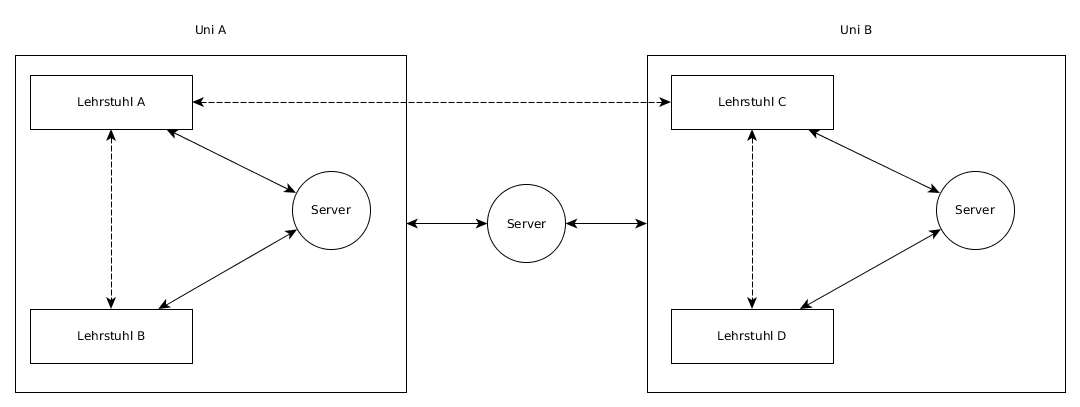
\includegraphics[width=\textwidth]{Masterarbeit_Bilder/Lehrstuhl_Datentausch_extern.png}
    \caption{Schematischer Aufbau des Universitätsnetzwerkes}
    \label{fig:ist-struktur}
\end{figure}    

Das Problem der ,,Uni'' lässt sich bereits auf einen Lehrstuhl reduzieren, wie  die Abbildung \ref{fig:ist-struktur2} schematisch aufzeigt.
Auf den als ,,Server'' gekennzeichneten Objekten werden diverse Dienste wie Datenspeicherung oder E-Mail ausgeführt. Ein Arbeitsbereich enthält dabei Endgeräte, die über unterschiedliche Protokolle (HTTP, SMTP, IMAP, \ldots) mit den Server kommunizieren.

\begin{figure}[htbp] 
	\centering
	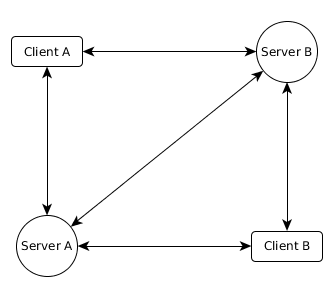
\includegraphics[width=0.65\textwidth]{Masterarbeit_Bilder/Lehrstuhl_Datentausch_intern.png}
	\caption{Schematischer Aufbau eines Lehrstuhls}
	\label{fig:ist-struktur2}
\end{figure}  

 Ein Server wie in Abbildung \ref{fig:ist-server} stellt Dienste zur Verfügung und unterscheidet sich von einem Endgerät wie in Abbildung \ref{fig:ist-endgeraet} nur geringfügig durch die verwendeten Programme. Die traditionelle Sicht, ein gegen den Ausfall besser abgesicherter Computer, wird immer seltener verwendet und ist im Rahmen der Arbeit nicht gefordert.
 
\begin{figure}[htbp] 
	\centering 
	\begin{minipage}{.5\textwidth}
	\begin{tabular}{|p{.9\textwidth}|}
		\hline
Server\\ \hline\hline
\\
NFS | SMB| Appeltalk | \ldots \\ \hline
Betriebssystem \\ \hline
Netzwerk (TCP /IP) \\ \hline
	\end{tabular}
	 
	\caption{Server}
	\label{fig:ist-server}
\end{minipage}%
\begin{minipage}{.5\textwidth}
	\begin{tabular}{|p{.9\textwidth}|}
 		\hline
		Client \\\hline\hline
		Browser \\ \hline
		Netzwerklaufwerk | \ldots \\ \hline
		Betriebssystem \\ \hline
		Netzwerk (TCP /IP) \\ \hline
	\end{tabular}
	\caption{Endgerät}
	\label{fig:ist-endgeraet}
\end{minipage}%
\end{figure}   
Die Plattformunabhängigkeit beachtet dabei die bekanntesten Betriebssysteme, zu denen gehören Linux (Fedora, Debian, \ldots), Windows und Mac OS. Zur Vereinfachung beziehen sich die Begriffe  \acrshort{nfs}, Web-Browser, Dateisystem und Dateimanager nachfolgend auf die jeweiligen vom Betriebssystem als Standard genutzten Anwendungen.

Für die nachfolgenden Szenarien wird eine Konfiguration wie in Abbildung \ref{fig:ist-struktur2} vorausgesetzt, bei der auf einem von Anwendern bedienten Endgerät ein Netzwerklaufwerk oder eine Festplatte als Datenspeicher verbunden ist. Neben einem Benutzernamen muss den Anwendern eine E-Mail-Adresse zugeordnet sein, um das Benachrichtigungssystem zu nutzen. Diese Voraussetzung kann schon beim Anlegen durch den Anwender selbst oder durch einen Administrator nachträglich erfüllt werden.


\subsection*{Suche über den Datenbestand}
Durch Eingabe von Schlagworten oder teilen des Dateinamen kann der Datenbestand durchsucht werden. Das anschließende Auswerten der Ergebnisliste zeigt folgende Probleme auf:

\begin{itemize}
	\item Lange Suchzeiten, wenn keine Datenbank mit Indizierung verwendet wird.
	\item Kaum Unterstützung bei der Suche, meist keine Verwendung der Verschlagwortung oder nur eingeschränkt nutzbar. 
	\item Benutzerinterfaces unterscheiden sich in der Unterstützung je nach verwendeter Plattform.
	\item Bei Verwendung ,,erweiterter Attribute'' gibt es nicht überall passende Unterstützung innerhalb des \acrshort{nfs} oder Dateisystems.
\end{itemize}

\subsection*{Zugriff auf den Datenbestand}
Mit bekannten Dateinamen wird auf das entsprechende Netzwerklaufwerk zugegriffen, um anschließend mit der gewünschten Datei zu arbeiten.

\bigskip
Folgende Probleme können anhand des Szenarios festgehalten werden:
\begin{itemize}
	\item Die meisten Funktionen, wie direktes Arbeiten auf einer Datei, sind Plattform abhängig. Daher unterscheidet sich die Arbeitsgeschwindigkeit von Anwendungen erheblich zwischen den Plattformen.
	\item Bei langen Dateipfaden ist das Navigieren komplexer und dadurch zeitaufwändiger.
\end{itemize}


\subsection*{Synchronisation der Daten}
Soll der Datenbestand von mindestens zwei Servern abgleichen werden, suchen diese untereinander nach nicht vorhandenen Dateien, um diese zu übertragen.

\bigskip
Folgende Probleme können anhand des Szenarios festgehalten werden:
\begin{itemize}
	\item Bei unterschiedlich großen Datenspeicher,\\
    - können Datenbestände eines Servers von unterschiedlichen Servern stammen.\\
    - müssen Datenbestände eines Servers ggf. auf mehrere Server aufgeteilt werden.
	\item Durch unterschiedliche Protokollabläufe in einem heterogenen Netzwerk ist die optimale Geschwindigkeit selten gewährleistet.
\end{itemize}
 
\subsection*{Zusammenfassung}
Die Arbeitsumgebung umfasst als Datenspeicher neben RAID-Systemen auf Servern, USB-Laufwerke sowie Netzwerkspeicher wie \acrshort{cifs} oder \acrshort{nfs}. Wegen der geforderten Plattform Unabhängigkeit, den verschiedenen Dateisystemen, folgen starke Abweichungen in Funktionalität und Unterstützung von Dateisuche und Dateizugriff.

Eine Annahme für die Arbeit ist, dass auf den Endgeräten ein Webbrowser und E-Mail-Client (mindestens eine Webschnittstelle) bereitgestellt wird.

Die Anwender nutzen weiterhin entsprechenden ,,Netzwerklaufwerke'', um mit den Dateien zu arbeiten.
Ein Übertragen dieser ist wegen der Größe aus Zeitgründen nicht akzeptabel. Dem Anwender ist dafür mindestens ein Benutzerkonto mit E-Mail-Adresse zugewiesen, um sich auf den entsprechenden Servern anzumelden. 

\bigskip
Es ergeben sich Anforderungen für die Realisierung wie:
\begin{itemize}
\item Zuordnung einer Person zu den diversen Konten an den entsprechenden Servern und Endgeräten
\item Auslesen der Informationen einer Datei unter Beachtung des Dateisystems
\item Zuordnung einer Datei zur entsprechenden Person als Verantwortlicher
\item Anzeigenanpassung und individuelle Unterstützung je nach verwendeter Plattform
\item Übertragung der Dateien zwischen teilnehmenden Computern
\item Benachrichtigungen über Dateizustände
\item Persistente plattformunabhängige Speicherung der Dateiinformationen 
\item Verlinken der \acrshort{dms}
\end{itemize}
 


\chapter{Grundlagen und verwandte Ansätze}
\chapmd{Albert Einstein (1879--1955)}{,,So einfach wie möglich. Aber nicht einfacher!''}

In der Einleitung werden Anforderungen, Annahmen und Umfeld der Anwendung skizziert.
Um das ,,wie'' zu klären, wird in diesem Kapitel ein Überblick über diverse Dateisysteme gegeben, Möglichkeiten der Kommunikations-Realisierung gezeigt und bestehende kommerzielle Lösungen einander gegenübergestellt.

\section{Betriebssystemabhängige Verschlagwortung}
In der Einleitung wird bereits darauf verwiesen, dass auf allen Plattformen eine grundlegende Unterstützung für die Verschlagwortung von Dateien existiert. Die Realisierung erfolgt meist durch Verwendung ,,erweiterter Attribute'', die ursprünglich zur Verwaltung der Benutzerrechte verwendet wurden. 

Seit ,,Windows Server 2008'' erfolgt dies zudem zur Abbildung der Rechte in heterogenen Netzwerken durch den Domain-Controller  \cite{windowsserver2008}.

Seit dem Jahr 2004, mit Kernelversion 2.6, nutzt Linux erweiterte Attribute, welche auch eingesetzt werden, um ,,Dateien leichter zu finden''  \cite{von2006100}. Beschränkungen in der Verwendung sind unter Linux jedoch am stärksten. Beispielsweise auf Dateisystemen mit Ext2 Basis in die Größe der Schlüssel-Wert-Paare. Im Fehlerfall kann eine Meldung wie

\begin{quote}
attr\_set: Auf dem Gerät ist kein Speicherplatz mehr verfügbar
\end{quote}

auftreten. Da die Möglichkeiten der Speicherung innerhalb einer INODE der Datei begrenzt ist \cite{kernelwiki}.

Durch eine geeignete Abstraktion ist mit Einschränkungen dennoch möglich eine Betriebssystem übergreifende Lösung zu realisieren. Das Entwickler-Team rund um Samba beweist dies mit ihrer Implementierung des Windows Netzwerk Dienstes. Die Entwickler weisen jedoch auf die Limitierungen in den Dateisystemen auf POSIX Systemen hin  \cite{smb}.

Windows und OS X unterstützen ,,erweiterte Attribute'' durch Technologien wie ,,\acrfull{ads}'' bzw.  ,,\acrfull{rf}'' besser und vermeiden so die meisten Beschränkungen \cite{surendorf2010mac}. Unter OS X sind zudem durch das Dateisystem HFS+ weniger Beschränkungen begründet \cite{macdsa}.

Jedes der zuvor genannten Betriebssysteme verwendet eigene Systemtools zur Verwaltung der ,,erweiterten Attribute'' sowie den darauf aufbauenden Diensten. Die Umsetzung einer einheitlichen Suche ist durch die Abweichungen des Funktionsumfangs der Betriebssysteme erschwert.

Die Programmiersprache Java hat erst mit Version 7 auf den gestiegenen Bedarf reagiert und versucht Attribute einheitlich abzubilden. So wird je nach Plattform und Dateisystem ein passendes ,,AttributeView'' gewählt, um Funktionalitäten optimal zu nutzen \cite{javanio}.

Bei Problemen mit der Kodierung kann durch Verwendung von UTF-8 auf diese entgegengewirkt werden.
Die genannten Einschränkungen bleiben bei der Speicherung dennoch erhalten: Da keine geeignete Implementierung unter Linux existiert, die vergleichbar mächtig  wie \acrshort{ads} oder \acrshort{rf} ist. Daher muss auf möglichst wenig Speicherung innerhalb der Datei geachtet werden, um Plattformübergreifend mit gleicher Funktionalität zu arbeiten.

  

\section{Speicherung sehr großer Daten}

Das Dateisystem unter OS X ist vorzugsweise {HFS+}, weitere Dateisysteme wie {FAT}, { NTFS} (Windows), {ZFS} (Solaris/BSD), {Ext4} (Linux) können durch entsprechende Treiber bei Bedarf nachinstalliert werden \cite{winext}, \cite{macntfs}. Das ist genauso für Windows zutreffend, jedoch mangelt es an produktiven Implementierungen anderer Dateisysteme. So das Nachfolgend von den jeweiligen bevorzugten Dateisystemen auf den Plattformen ausgegangen wird.

Ab Mac OS X v10.5.3 unterstützt  {HFS+} bis zu 8 Exabytes \cite{maclimit}. In direktem Vergleich mit Linux Ext4, welches maximal im Petabyte Bereich Daten speichern kann, ist HFS+ zukunftssicherer entworfen \cite{kernelwiki}.

Die meisten Distributionen von Linux unterstützen maximal ein Exabyte je Datei. Das soll sich erst ändern, wenn das als Linux Dateisystem angepriesene {Btrfs}, welches bis zu 16 Exabyte verwalten kann, veröffentlicht wird \cite{btrfs}. Es ist jedoch möglich, ZFS in Linux zu verwenden, welches bevorzugt in Solaris und FreeBSD eingesetzt wird \cite{zfslinux}.

NTFS bietet als das Windows-Dateisystem nur theoretische 16 Exabyte, da die Implementierung lediglich 16 Terabyte unterstützen \cite{ntfslimit}. Ältere Dateisysteme wie {FAT} enden bereits mit knapp 4 Gigabyte je Datei und fallen dadurch vollständig aus dem Kontext der Arbeit \cite{fatlimit}.
 
Die aktuellen Dateisysteme bieten alle Voraussetzungen, um wissenschaftlichen Daten entsprechend der Aufgabenstellung im Terabyte-Bereich zu verwalten. Da aktuelle Festplatten bei ca. 10 Terabyte enden, ist es nur mit einem \acrfull{lvm} möglich, sich den theoretischen Grenzen der Dateisysteme anzunähern. Dieser Manager stellt verschiedene RAID-Level bereit und ist teilweise direkt in die Hardware implementiert. Bei Softwareimplementierungen ist diese Fähigkeit unter {ZFS} oder {Btrfs} sogar schon auf Dateisystemebene vorhanden und muss nicht mehr durch entsprechende Dienste im System bereitgestellt werden \cite{zfsraid}.
Die Beschränkung der Festplatten kann dadurch umgangen werden.
Zu beachten ist allerdings, dass die Ausfallwahrscheinlichkeit erheblich steigt, je mehr Festplatten verwendet werden  und eine sichere Datenspeicherung mit zunehmender Größe schwer wird.Da es keine Patentlösung für ein passendes RAID-Level gibt, muss je nach System und Anwendung ein Konsens zwischen Sicherheit, Speicherkapazität und Geschwindigkeit gefunden werden.

Zusammenfassend kann festgehalten werden, dass für die Dateispeicherung {ZFS} und {HFS+} im Jahr 2015 die besten funktionalen Voraussetzungen bietet, die für einen stabilen Betrieb notwendig sind. 


\section{Kommunikation in verteilten Anwendungen}\label{sec:comm}
Bei der Kommunikation und  dem Datenaustausch in verteilten Anwendungen können verschiedene Ansätze verfolgt werden. Eine auf Nachricht basierte Kommunikation ist wegen der großen Zeitfenster infolge der Dateigröße das Sinnvollste.

Zur Realisierung eines \acrfull{rpc} bieten daher Protokolle wie \href{http://xmpp.org/}{XMPP}  oder IRC einen ersten Ansatz.

Das Bootstrapping Problem beschreibt den erschwerten Einstieg in das P2P-Netzwerk. Bei IPv4 verstärkt sich diese Problematik durch eine mit \acrfull{nat} versehene Firewall und ist für die meisten \acrshort{p2p}-Netzwerke kaum überwindbar, obwohl meist externe Dienste unterstützend verwendet werden.

Mit IRC-Bootstrapping hat sich die Universität Duisburg-Essen bereits beschäftigt und löst die Beschränkung des Protokolls durch eine Zufallszahl im Chatnamen \cite{5159226},\cite{RFC2812}. Diese Problematik wird in aktuelleren Protokoll wie \href{http://xmpp.org/extensions/xep-0045.html\#enter-conflict}{,,XMPP XEP 45''} durch ,,resources'' gelöst.

XMPP sieht zwar eine \acrshort{p2p}-Übertragung vor, die mit ,,XEP-0066: Out of Band Data''  beschrieben ist. Deren Unterstützung durch Bibliotheken ist jedoch nicht vollständig. Daher wurde von einer Implementierung abgesehen.

Problematisch für beide genannten Dienste ist die Exklusivität für menschliche Interaktion. Administratoren blockieren Bots auf den Servern den Zugang und das Betreiben eigener Server ist aufwändig und für die Aufgabe nicht praktikabel.

 
\subsection{Java JXTA}
Führend in Java ist \href{https://jxta.kenai.com/}{{JXTA}} als ein reiner \acrshort{p2p}-Ansatz. Die Aussage von \href{http://www.vs.uni-due.de/}{Herrn Prof.\ Weis}:

\begin{quote}
Es ist billiger 10 Server zu finanzieren, um die Client-Server Anwendung laufen zu lassen, als einen Entwickler, der eine \acrshort{p2p}-Lösung programmiert.
\end{quote}
%% hier ruckelt es noch !!!
beschreibt die Komplexität, welche mit einer geeigneten Bibliothek zu minimieren versucht wird.
Die Problematik des veralteten IPv4 Netzwerkes ist hier versteckt und der eigentliche Grund, warum kaum \acrshort{p2p}-Lösung Verwendung finden.

Durch neuere Protokolle wie IPv6 sollen die größten Probleme, wie \acrshort{nat}, gelöst werden.
Jedoch ist IPv6 noch nicht überall vorhanden, dass es sich lohnt, einen solchen Ansatz zu verfolgen.
Sobald in Deutschland durchgängig IPv6 vollzogen würde, bedarf dieser Einschätzung einer erneuten Betrachtung. Nach der Google Statistik läuft diese Umstellung jedoch nur langsam \cite{gstat}. 


\subsection{SOAP, REST oder WebRTC}
Im Bereich der Webanwendungen existieren als Standardnachrichtenaustauschprotokolle {SOAP} und {REST}.
Die auf {XML} basierenden Protokolle werden in Webservices verwendet, um verteilten Anwendungen die Kommunikation zu ermöglichen.
Vorteilhaft ist dabei der Umstand, dass infolge der starken Verbreitung von {HTTP} durch Webserver Verbindungen kaum durch Firewalls blockiert werden. 
Bei {WebRTC}, welches mit {HTML5} eingeführt wurde, ist die P2P-Lösung greifbar nah. Dieser Standard, ist jedoch nicht bei allen gängigen Systemen implementiert \cite{cani}. So das dieser Ansatz nicht Zielführend ist.

In diesem Zusammenhang ebenfalls betrachtenswert wird {JSON} als eine Alternative zu {XML} gehandelt. Das Format wird vorzugsweise bei verteilten JavaScript Anwendungen eingesetzt und ist im Vergleich zu {XML} einfacher und kürzer. In vielen Programmiersprachen ist es -- durch Bibliotheken -- meist trivial, die Datenpräsentation entsprechend zu wechseln.


\subsection{Java Message Service (JMS)}
\label{chap:jms}
Beim \acrfull{jms} handelt es sich um eine ,,Message Oriented'' Middleware, welche die Kommunikation zwischen Programmen vereinheitlichen soll. Vergleichbare Ansätze finden sich im XMPP-Protokoll wieder. Realisiert wird eine lose Kopplung einzelner Programmteile durch Nachrichtenaustausch.

Neben der internen Java-VM Kommunikation wird eine {TCP/IP} Möglichkeit angeboten, die nicht nur von Java Anwendungen genutzt werden kann.

\bigskip

Durch ein Beobachter-Muster  wird ein Chatroom abgebildet, welcher durch Topic im  \acrshort{jms} realisiert ist.
Wie in den meisten Mehrbenutzerchats existiert keine Historie, so dass neue Teilnehmer nur Nachrichten erhalten, wenn diese angemeldet sind.

Anderes Verhalten weist eine Queue im \acrshort{jms} auf: Gespeicherte Nachrichten können dadurch später noch ausgelesen werden.

Das durch einen separaten Dienst bereitgestellte System fungiert als Vermittler zwischen Anwendungen und nutzt Javas interne Serialisierung zur korrekten Darstellung der Nachrichteninhalte.
 


\section{Kommerzielle/andere Lösungen}
Diese Arbeit versucht in ein bestehendes Netzwerk eine \acrshort{p2p}-Lösung zu etablieren, um ein Suchen von Dateien besser zu unterstützen. Einem Vergleich mit marktführenden Produkten wie  \href{http://www.alfresco.com/}{{Alfresco One}}, \href{https://www.powerfolder.com/de/powerfolder-erhalt-qualitatssiegel-it-security-made-in-germany/}{{PowerFolder}} oder \href{https://www.dropbox.com/de/}{{Dropbox}} kann diese Anwendung nicht standhalten.
Jedoch unterscheidet sich diese Software in einigen Aspekten von den genannten Produkten.

\subsection{Cloud Storage}
Im Bereich der Dateiverwaltung hört man schnell von Diensten wie \href{https://www.dropbox.com/de/}{{Dropbox}}, \href{http://www.openkm.com/en/}{{OpenKM}},
\href{https://onedrive.live.com/}{{Windows OneDrive}} oder  \href{https://www.google.com/intl/de_de/drive/}{{Google Drive}}.
Alle Dienste haben gemein, dass sie von sehr großen Unternehmen bereitgestellt werden und nahezu unendlich viel Speicherplatz anbieten. 

In der Unterstützung unterscheiden sich die Dienste teils gravierend voneinander. {Dropbox} bietet unter den Cloud Storage Diensten dabei vergleichsweise die beste plattformübergreifende Unterstützung.

Bei vielen Diensten wird die Plattform Linux kaum unterstützt. Hierbei handelt es sich häufig um nicht offizielle Anwendungen, die nur wenige Funktionen anbieten. \href{https://one.ubuntu.com/}{Ubuntu One} stellt für die Wenigsten eine echte Alternative dar, da der Dienst weder Verbreitung noch Integration in anderen Produkte besitzt. Bei {Google Drive} ist der Hinweis zu finden, dass die Linux-Unterstützung noch in Arbeit ist \cite{googledrive}.

{Dropbox} bietet auf den meisten Plattformen alle Funktionen gleichermaßen an, jedoch hat dieser Dienst Nachteile.
Bei dem Client lassen sich nicht mehrere verschiedene Ordner verwalten. Dadurch werden gewisse Datenstrukturen erzwungen, was nicht immer erwünscht ist und zu Problemen führen kann, wenn Anwendungen bestimmte Pfade benötigen.

Alle genannten Dienste haben für das Arbeiten mit wissenschaftlichen Daten den Nachteil, dass die Clients Dateien lokal synchronisieren. Da Verbindungen ins Internet immer noch langsam sind und die nötigen Transfer-Kapazitäten enorme Kosten verursachen, ist dieser Ansatz nicht praktikabel \cite{telekomlahr}. Der Vorteil einer Cloud basierten Lösung, dem einfacheren Teilen der Daten, wiegt diese Nachteile nicht auf.

Ein weiter wichtiger Aspekt ist die rechtliche Lage. Gerade im wissenschaftlichen Bereich gibt es viele Daten, die dem Lehrstuhl exklusiv oder durch eine bestimmte Rahmenbedingung bzw. Lizenz zu Verfügung gestellt werden. 
Daher ist es für viele Daten nicht möglich Cloud-Dienste wie Dropbox oder Google Drive zu verwenden. 
Das erstellte System lässt die Daten dort liegen, wo diese erstellt werden. Ein Synchronisieren erfolgt nur auf Wunsch durch die Anpassung der Konfiguration.

\subsection{Lokales Netzwerk}
Auch im lokalen Netzwerk sind die Cloud basierten Ansätze zu finden. Lösungsansätze mit einem FTP-Server sind von ihren Funktionen her, beim Dateiaustausch, nicht mehr zeitgemäß. Auch das Protokoll ist nicht dazu geeignet, konkurrierende Zugriffe auf Dateien zu verwalten.

Datentransfer im lokalen Netzwerk ist daher durch Technologien wie \acrshort{nfs} geregelt.
Diese Dienste lassen sich jedoch meist wegen ihrer Protokollbeschränkungen im Internet nicht nutzen.

Meist darauf aufbauend haben speziell im Bereich Verschlagwortung und kooperatives verteiltes Arbeiten, Groupware Lösungen wie \href{https://owncloud.org/}{{ownCloud}} oder \href{http://www.horde.org/apps/groupware}{{Horde}} den Begriff der privaten Cloud geprägt. Als Dateibrowser eignen sich diese Oberflächen jedoch kaum. Auch die geforderten Funktionen wie die Prüfsummenberechnung zur Erkennung von Duplikaten und Veränderungen ist in diesen nicht vorhanden.

Ein verteilter Ansatz lässt sich genauso wie die neuen Funktionen integrieren. Da die Anwendungen jedoch ,,Open-Source-Lösungen'' sind, benötigt die vorherige Einarbeitung in die Anwendung zu viel Zeit. 

Die meisten Anwendungen im Open-Source Bereich haben nur eine mangelnde Unterstützung der 64 Bit Architektur. Für PHP auf Windows heißt es auf der Webseite, dass ,,large file support'' noch immer nicht vernünftig funktioniert und 64 Bit nicht stabil läuft \cite{phpw}. Diese Limitierung gilt dabei genauso für Horde und ownCloud, welche in PHP programmiert sind. Eine Implementierung der nötigen Funktionen kann wegen den Anforderungen nur schwerlich auf 32 Bit erfolgen. Inwieweit Konzepte wie \acrfull{pae} berücksichtigt werden können, muss noch evaluiert werden. Die 32 Bit Unterstützung ist aber nicht Gegenstand dieser Arbeit.
Da Java 64 Bit unterstützt, wird hier bei Verwendung sehr großer Dateien auf diese Technologie zurückgegriffen.

{OpenKM}, wie Abbildung \ref{openkm:home} zeigt, ist einer Lösung des in der Einleitung beschriebenen Problems nah, jedoch sind hier immer noch nicht die genannten Funktionen wie die Berechnung der Prüfsumme ersichtlich. Diese sind wie bei  {Alfresco One} gegen passende Bezahlung integrierbar, da beide Systeme kommerziell vertrieben werden.

Ein weiterer Nachteil ergibt sich aus dem Laden der Dateien. Statt diese durch entsprechende Links im System zu öffnen, wird ein Terabyte Download über HTTP gestartet. 

\begin{figure}[htbp] 
    \centering
    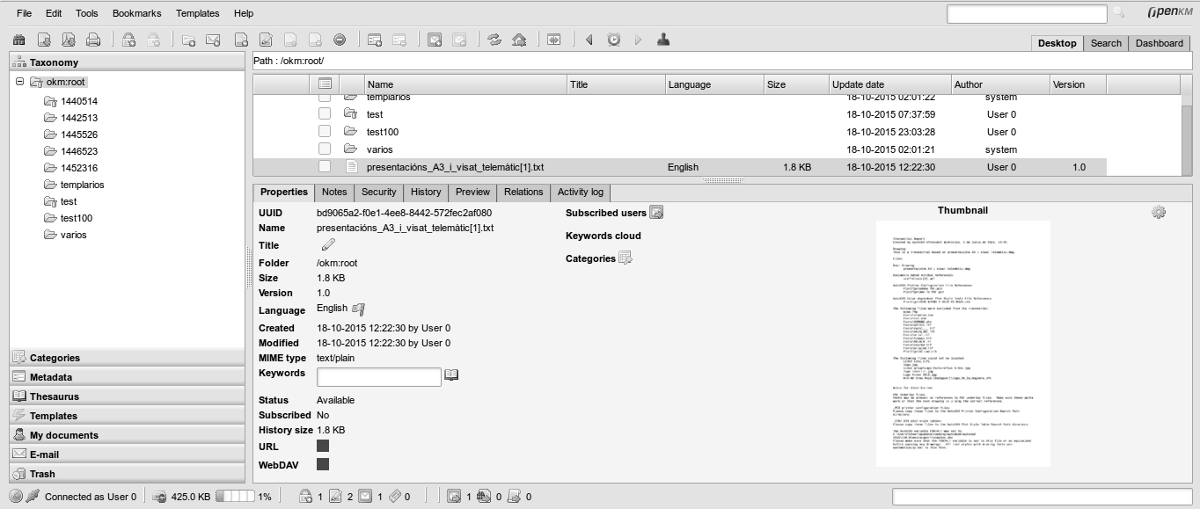
\includegraphics[width=\textwidth]{Masterarbeit_Bilder/openkm.png}
    \caption{Startseite der Webanwendung OpenKM}
    \label{openkm:home}
\end{figure}  


Das hier erstellte System nutzt einen anderen Ansatz zur Datenbeschaffung und Datensuche. Diese Suche beschränkt sich im Rahmen dieser Arbeit auf einfache Mustervergleiche und erlaubt das Suchen von Dateien über mehrere Peers hinweg anhand gesammelter Meta-Informationen. 
Der Dateizugriff erfolgt dabei durch ein Script mit entsprechender Konfiguration auf dem Endgerät, was einen Download vermeiden kann.



\chapter{Technische Analyse}
\label{chap:techAnal}
\chapmd{ Eine Weisheit der Dakota-Indianer}{,,Wenn Du entdeckst, dass Du ein totes Pferd reitest, steig ab.''}
 
Auffällig ist, dass die meisten plattformübergreifend \acrshort{dms}-Systeme mit ,,großen'' Dateien in Java programmiert sind. Das Nutzen von HTTP zeigt bei großen Dateien schnell schwächen und dadurch aufkommende Probleme bleiben ungelöst. Das zeigt sich in der Nutzung von WebDAV sowie bei Downloads \cite{davlimit}, \cite{httplimit}.

Es muss das richtige Protokoll für den jeweiligen Anwendungszweck verwendet werden, was jedoch nicht immer durch die verwendete Architektur umsetzbar ist. 
Der in dieser Arbeit verfolgte Ansatz ermöglicht eine flexible Gestaltung der Protokolle im Dateiaustausch.
\section{Warum Java}
Die plattformunabhängigen Anwendungen nutzen naheliegenderweise Java als Programmiersprache. Auch Scriptsprachen verwenden neben passendem Interpreter, meist in C/C++, die Java Plattform, dessen bekannteste Vertreter Python und Ruby sind.
Seit Java Version 7 ist die Einschätzung von James Gosling ,,Java ist wie C++ ohne Pistolen, Messer und Clubs." technisch nicht mehr haltbar, da mit Einführung von Java 8 und den Funktionalitäten, wie z. B.  \href{http://www.oracle.com/technetwork/articles/java/trywithresources-401775.html}{,,automatic resource management''} und \href{http://www.oracle.com/technetwork/articles/java/rich-client-lambdas-2227138.html}{,,Lambda''}, die Möglichkeit geschaffen wurde, andere Programmierkonzepte in der Sprache zu verwenden.

Auch für die Programmierung von Weboberflächen bietet Java mit \href{http://www.oracle.com/technetwork/articles/java/enterprise-html5-2227136.html}{JSF und HTML} eine schnelle und einfache Möglichkeit, Web-Anwendungen zu erstellen.

Die riesige Entwicklergemeinde hat viele Bibliotheken hervorgebracht, deren Ergebnisse heute in anderen Sprachen zur Anwendungsrealisierung verwendet werden. Die bekanntesten von ihnen werden von der
\href{http://www.apache.org/}{ ,,Apache Software Foundation'' } gepflegt.


%% stolpern hier ....
Was Windows dieses Jahr mit {.NET} startete, hat Java lange zuvor durchgeführt. Durch die gemeinsame Open-Source Basis und der Möglichkeit, die Virtuelle-Maschine legal mit in sein Programm zu integrieren, erlaubt eine sehr einfache Anwendungsbereitstellung und Erstellung eingebetteter Anwendungen. Nachfolgend bezieht sich die technische Analyse auf die Realisierbarkeit in einer Java Anwendung.


\subsection{Arbeiten mit Dateien}
Bei der Realisierung und dem Arbeiten mit Dateien gibt es trotz plattformunabhängiger API Schwierigkeiten. Ursachen sind Verhaltensunterschiede im Betriebssystem.
Es gibt allerdings grundlegende Informationen, wie dem Dateinamen, Dateipfad, Größe oder letzte Änderung, die sich auf allen Plattformen finden lassen.

Bei der Verschlagwortung handelt es sich um ein Anhängen von Informationen. Diese Informationen sind bei der Speicherung nicht nur plattformabhängig, sondern unterscheiden sich bereits erheblich innerhalb des verwendeten Dateisystems einer Plattform.
Die meisten Betriebssysteme nutzen dabei ,,erweiterte Attribute''. Inwieweit auf Mac OS ,,\acrshort{rf}'' und auf Windows ,,\acrshort{ads}'' Verwendung findet, wurde nicht geprüft.  
 
Die einfach klingende Idee, Rechenzeit zu sparen, indem Informationen voranalysiert und an die Datei anhängt werden, kann jedoch schnell durch einen Anwender oder ,,falsch'' funktionierendes Programm komplex sein. Am Beispiel von Prüfsummen zeigen sich die Probleme bereits lokal auf dem Computer. Dazu berechnet ein Programm zu einer gegebenen Datei eine Prüfsumme und hängt das Ergebnis der Berechnung an die Datei an. Hier muss davon ausgegangen werden, dass das Dateisystem ebenso wie das Betriebssystem alle nötigen Funktionen bietet.

\bigskip
Folgende Ergebnisse können eintreten:
\begin{itemize}
	\item Änderungen an der Datei sorgen für eine nicht mehr gültige Prüfsumme in den Attributen.\\
    Lösung: Durch Nutzung von Zeitstempel, der Prüfsummen, kann bei Abweichungen des Prüfsummen-Zeitpunktes zum Modifikationsdatum die Prüfsumme neu berechnet werden.
    
	\item Verpassen von Dateimodifikationen.\\
     Lösung: Sollte der Verdacht existieren, dass sich die Datei geändert hat, ohne Änderung im Änderungsdatum, sollte eine neue Berechnung erzwingbar sein.
     Auslöser könnten Programme sein, die neben dem Dateiinhalt deren Meta-Informationen verändern. Wie mit diesem Problem umgegangen werden sollte, ist der Aufgabenstellung nicht zu entnehmen. 
     Durch eine Aktualisierung z. B. mit \verb|touch FILE| unter Linux wird das Modifikationsdatum erneuert was zu einem Neuberechnen führt.
     Dies kann als ,,externer''-Befehl in der Anwendung konfiguriert werden.
     
\end{itemize}

Wird davon ausgegangen, dass die verwendeten Programme Dateien nur mit ,,echten'' Änderungen neu schreiben oder erweitern, so ist es naheliegend, einen Prozess zu entwickeln, der die Änderungen bei Auftreten verarbeitet.

Es gibt zwei mögliche Ansätze zur Realisierung: {Polling} oder {Interrupt}. Nachteile beim Polling sind unregelmäßiges Reagieren auf Änderungen und Erzeugung von zu viel CPU-Last. Ein weiterer Nachteil ist, dass zu schnell hintereinander erfolgte Änderungen übersehen werden können.

Für das Nutzen von {Interrupts} muss das Betriebssystem passende Schnittstellen bereitstellen. Ein {Interrupt} wird anschließend für ein bestimmtes Ereignis, wie Erstellen oder Ändern einer Datei, angemeldet und vom Betriebssystem sowie von der passenden Hardware verwaltet. Im Fall der Dateiüberwachung wird von den meisten Betriebssystemen eine Ordnerüberwachung angeboten, die sich dem gewünschten Vorhaben, beispielsweise durch Filterung, anpassen lässt. Dieser Ansatz verpasst keine Änderungen und benötigt kaum CPU-Rechenzeit.


\section{Kommunikation}
Im Abschnitt (\ref{sec:comm}) wurden zwei der größten Vertreter zur Kommunikation genannt. Realisiert ist die Anwendung unter \acrshort{jms}, anders als  \href{http://xmpp.org/extensions/xep-0060.html}{,,XMPP (draft) XEP60''} stellt dieses eine etablierte Kommunikationsschnittstelle bereit, in der eine nachrichtenbasierte verteilte Anwendung programmierbar ist.

Zwischen Anwendungsserver und Client wird HTTP verwendet, um HTML Dokumente auszuliefern. Die Implementierung erfolgt auf Grundlage von HTTP 1.1. Kommende Versionen wie Java 9 nutzen bereits das von Google vorangetriebene HTTP 2 \cite{httpx1}, \cite{httpx2}. Es ist jedoch nicht vor Mai 2016 mit einer verwendbaren Veröffentlichung zu rechnen.

Die Clients selbst sprechen  (Abbildung \ref{fig:ist-struktur2}) zwischen den jeweiligen Servern bereits ein geeignetes Protokoll für den Datentransfer. Daher ergibt sich in der Kommunikation eine heterogene Landschaft, die die Vorgabe erfüllt, skalierbar zu sein. Davon ausgehend, dass der Dateitransfer zwischen Server und Client durch das passende vom Betriebssystem empfohlene Protokoll skalierbar ist. Wird auf weiterführende Literatur verwiesen, um den hier verwendeten Anwendungsserver zu skalieren und beispielsweise im Cluster zu betreiben \cite{glassfishcluster}.
Die hier erstellte eingebettete Version unterstützt allerdings keinen Cluster Betrieb und erfordert für eine Lastverteilung mehr Konfigurationsaufwand auf den einzelnen Peers. Nachteilig ist die dadurch entstehende höhere CPU- und RAM-Last.
 
\section{Sicherheit}
Im Punkt Sicherheit wird auf externe Dienste wie SSH oder VPN verwiesen.
Die Anwendung verwendet keine Verschlüsselung im eingebetteten Modus. Üblicherweise muss dazu ein ,,selbst signiertes Zertifikat'' erzeugt werden, welches i. d. R. von Webbrowsern als nicht vertrauenswürdig angezeigt wird. Dies macht, für einen reibungslosen Betrieb, ein vorheriges Verteilen des Zertifikates und dessen Installation notwendig. Die nötige Arbeit entsprechender Realisierung wurde in andere Aufgabenbereiche verlagert. Die grundlegenden Algorithmen werden bereits durch die Bibliothek der ,,Legion of the Bouncy Castle'' bereitgestellt und kann bei Bedarf integriert werden\cite{javabc}.

Ein Ausführen der Webanwendung über einen Proxy mit \acrfull{tls} Verschlüsselung ist jedoch einfach.

Ebenso kann eine Nachricht vom \acrshort{jms} durch Nutzung von beispielsweise SSH-Port-Weiterleitungen versendet werden. Diese Dienste sind weitgehend transparent für die Anwendung nutzbar.
Die Kommunikation mit einem E-Mail-Server erfolgt über Javas interne \acrshort{tls},  da hier ein ,,vollständiger'' Client implementiert ist. Die Anwendung akzeptiert Standardmäßig alle Zertifikate und umgeht dadurch die Schutzmechanismen, da auf den Testsystemen keine ,,echten'' sondern nur selbst signierte Zertifikate vorliegen.
Diese Prüfung kann mit entsprechender Konfiguration geändert werden, so dass nur noch konfigurierte Zertifikate und ,,Hosts'' erlaubt sind. Dazu muss das Java-Tool ,,keytool'' verwendet werden, um dem Java System entsprechende Zertifikate mitzuteilen.

Sicherheitstechnisch bedenklich ist, dass ein Peer, welcher sich zu einem Server verbindet, diesem vollständig vertraut.
Selbst wenn die Kommunikation zwischen den Peers sicher gestaltet ist, kann die Anwendung durch Konfigurationsschwächen und Anforderungen wie der Befehlsausführung, der Vorfilterung von Daten, durch externe Prozesse, über die  Weboberfläche erhebliche Sicherheitslöcher in die bestehende Netzwerklandschaft reißen.

Der abhörsichere Transport und die Sicherheit in der Kommunikation unter den Peers geht dabei weit über die eigentliche Aufgabe hinaus und muss getrennt betrachtet werden. Um sich für eine geeignete Sicherheit entscheiden zu können, muss das System jedoch erst getestet werden. Ein ,,public/private key'' Verfahren könnte dabei genauso wie das Erzeugen einer zentralen Zertifizierungsstelle in das erstellte System etabliert werden.

Bis zu einer entsprechenden Entscheidung sollte das System bei Bedarf durch TLS Proxy oder HTTPS aus einem anderem Webserver, außerhalb des eingebetteten Modus, oder durch SSH-Port-Weiterleitungen.


 
%%  ----- NEW ----



\section{Anwendungsserver}
\label{chap:appserv}
Die Anwendung baut auf etablierten Bibliotheken im Java Umfeld auf. Als Server im eingebetteten Modus wird ,,Glassfish'' verwendet.
Lösungen mit Tomcat oder Jetty konnten wegen der JSF-API nicht verwendet werden, da viele genutzte Funktionen nicht vorhanden sind und es mehr Aufwand bedeutet, diese zu integrieren. Neben der gängigen Internet-Literatur gibt es Bücher, die das Einrichten und die ersten Schritte beschreiben wie \cite{glassfishee7}. Da sich aber für das Einbetten in die Anwendung beim ,,master'' entschieden wurde, werden nötige Konfigurationen vom Programm selbst erledigt.
Die Entscheidung für einen eingebetteten Anwendungsserver ist darin begründet, dass die Administration möglichst einfach gehalten werden soll.
Die Installation eines Anwendungsserver benötigt einen großen Konfigurationsaufwand und ist für normale Anwender ohne Vorwissen und Grundlagen nicht möglich.


\subsection{Webanwendungen}
Heutige moderne webbasierte Anwendungen im Java Umfeld werden mittels {JSF} erstellt. So kann sich ein Java-Entwickler auf Java fokussieren und muss sich nicht hauptsächlich mit den Anforderungen von HTML und Javascript auseinandersetzen, da viele notwendige Scripte und Elemente automatisch erzeugt werden. HTML5 stellt nicht alle Eingabeelemente wie vom Desktop bekannt bereit. Meist werden diese durch Implementierungen wie \href{http://primefaces.org/}{{Primefaces}} ergänzt. Diese nutzen meist gängige CSS- und JavaScript-Bibliotheken wie \href{http://getbootstrap.com/}{Bootstrap} und \href{https://jquery.com/}{jQuery} für erweiterte Eingabeelemente und visuelle Effekte.

Mit JSF  werden vorzugsweise HTML-Seiten generiert und das binding Konzept vereinfacht das Entwickeln in Java.
Mit bindings lassen sich Objekteigenschaften an HTML-Elemente koppeln, so dass das Zurückspeichern der über HTTP übertragenen Daten nahezu automatisch erfolgt.

\subsection{Contexts and Dependency Injection}
%%--monstersatz
Bei \acrfull{cdi} werden Objekte verwaltet und dadurch die Möglichkeit geschaffen, Abhängigkeiten, die zur Laufzeit entstehen, im Betrieb einzufügen und erst anschließend die entsprechende Methode aufzurufen. Dadurch lassen sich viele Entwurfsmuster wie z. B. das Interceptor-Muster einfacher implementieren. Dafür müssen nur die entsprechenden Notationen an die Methoden geschrieben werden \cite{schmidt2002pattern}, \cite{gamma2011entwurfsmuster}, \cite{bien2003j2ee}. Das Interceptor-Muster lässt sich für das Einbauen von transparenten Transaktionen oder Log-Meldungen verwenden. Nachteil ist die schwere Nachvollziehbarkeit der Programmabläufe, da nicht wirklich klar ist, was an einer bestimmten Stelle injiziert wird.

Es ist darauf zu achten, dass alle Objekte im sogenannten {CDI-Kontext}, vom CDI-Container, meist innerhalb des Anwendungsserver, verwaltet werden. Neue Objekte, müssen durch entsprechende Notationen vom Container angefragt werden und werden nicht wie üblich durch ,,new'' erzeugt.

\bigskip
Die wichtigsten Muster für die Realisierung sind:

\begin{itemize}
    \item Interceptor, \cite{schmidt2002pattern}
    \item Dekorator-Muster, \cite{gamma2011entwurfsmuster}
    \item Chain-of-Responsibility, \cite{gamma2011entwurfsmuster}
    \item Proxy-Muster, \cite{gamma2011entwurfsmuster}
    \item Data Access Object (DAO) Muster, \cite{bien2003j2ee}
\end{itemize}

Werden {CDI}, {JSF}, {JPA} in einer Anwendung verwendet, ergeben sich Synergien. So können Konfigurationen von Datenbanken lose gekoppelt werden und deren Transaktionen bei Bedarf durch einen Interceptor gestartet werden. Programme die {CDI} und {JPA} einsetzen, verwenden meistens das ,,Data Access Object''-Muster, welches notwendige Funktionen zum Datenspeicher nochmals vor der speichernden Anwendung kapselt. Es wirkt dadurch als Fassade vor der Datenbank und stellt sicher, dass nicht jedes Objekt eine eigene Suche implementiert und damit doppelten Code erzeugt.

Die Kombination von {CDI} und {JSF} vereinfacht die Verwendung von ,,Java Beans'', indem in andere Objekte Eigenschaften injiziert werden können. Diese Flexibilität ist bei Webanwendungen und deren Formularen sehr wünschenswert, da einerseits Browser-Weichen so indirekt durch Muster wie  ,,Chain-of-Responsibility'' einem ,,richtigen'' HTML-Generator übergeben werden können und andererseits durch das ,,lifecycle management'' Session- und Request-Kontexte einfach verwendbar werden. 

Durch die Aktualität von Java 8 treten Probleme im Zusammenspiel mit nicht aktualisierten Bibliotheken auf. Es werden wegen den neuen Streams Konzepten von Java 8 beim Evaluieren falsche Referenzen verwendet, was zu einer ,,Nullpointer Exception'' führt. Kontexte mit Javas ,,Lambda'' Funktionen, sofern diese etwas komplexer sind, führen daher zu falschem Verhalten in der Anwendung.
An dieser Stelle muss von der Verwendung von Java 8 Konzepten teilweise abgesehen werden, bis die Implementierungen des Containers die neuen Sprachelemente vernünftig unterstützen.




\subsection{Java Persistence API}
\label{chap:jpa}

Das \acrfull{jpa} kann alternativ ergänzend zu {JDBC} eingesetzt werden und dient in Java Anwendungen der Datenbankkommunikation. Das darin integrierte \acrfull{orm} ermöglicht Tabelleninhalte in Objekte zu überführen. Durch Notationen an den Java-Klassen wird die XML basierte Konfiguration auf ein Minimum beschränkt und die nötige ,,persistence.xml'' enthält teilweise nur die Verbindungsdaten zur Datenbank.

Vorteile der Notationen im Code gegenüber der alten {XML} basierten Konfiguration ist die Möglichkeit der Prüfung durch den Compiler. Javas integrierte Zyklenerkennung wird beim \acrshort{orm} verwendet, um bei komplexeren Datenstrukturen redundante Speicherung zu vermeiden \cite{inden2012weg}.


%% -- ralf?
Der effizienteste Ansatz ist das Erweitern einer Klasse für direktes Arbeiten auf der Datenbank. Das kann durch die Bibliothek während des Compilierens oder zur Laufzeit erledigt werden. Vergleichbare  Lösungsansätze müssen sich der Reflection-API behelfen und Verfahren wie die Zyklenerkennung meist selbst entwerfen.
Optimierungspotential gibt es zudem durch angepasste SQL-Ausdrücke und der Nutzung von Datenbank spezifischen Funktionen.

Die Problematik, dass in jedem Objekt die Datenbankinformationen ständig mit gespeichert werden, wird mittels {,,detach''} Operation vermieden. Dadurch wird auf die Objektverwaltung und Funktionen wie dem ,,lazy loading'', welche Daten erst bei Bedarf von der Datenbank liest, verzichtet, was in Anwendungen, die große Datenmengen verarbeiten, viel RAM spart und die Anwendung beschleunigt.

Im  Zusammenhang mit Java 8 sind bei \acrshort{jpa} Probleme zu finden. Hier muss wiederum bedingt durch die Bibliothek gänzlich auf Java 8 verzichtet werden.
Dies liegt an der internen Erweiterung von Java-Klassen. Mit \href{http://openjpa.apache.org/openjpa-2.4.x.html}{OpenJPA 2.4} wurde eine Java 8 Unterstützung implementiert. Der verwendete Anwendungsserver ist jedoch mit \href{http://www.eclipse.org/eclipselink/}{EclipseLink} ausgestattet und die neue Version mit Java 8 Unterstützung erst am 30.9.2015 erschienen, so dass zum Planungszeitpunkt keine entsprechende Unterstützung existierte.




\chapter{SCISERVER}
\chapmd{ Johann Wolfgang von Goethe (Werk: Wilhelm Meisters Wanderjahre)}{,,Es ist nicht genug, zu wissen, man muss auch anwenden; es ist nicht genug, zu wollen, man muss auch tun.''}


In diesem Kapitel wird die Anwendungsrealisierung beschrieben. Sicherheitsaspekte und Verschlüsselung muss durch externe Anwendungen eingebunden werden. Die Nutzung von SSH ist ratsam. Interne verwendete Verschlüsselungsverfahren dienen lediglich zur Authentifizierung. Die Anwendung wurde in mehrere Projekte strukturiert und durch das Build-Tool \href{https://maven.apache.org/}{{Maven}} kann das Projekt in allen gängigen \acrshort{ide} entwickelt werden. 


\bigskip
Ein Rückblick auf die Zusammenfassung zeigt, wie welche Aufgaben von der Anwendung erfüllt werden:

\begin{itemize}
     \item Zuordnung einer Datei der entsprechenden Person als Besitzer/ Verantwortlicher sowie zu den diversen Konten an den entsprechenden Servern und Endgeräten.
     
    Die Dateibesitzer-Informationen werden aus den Dateien ausgelesen und durch die manuelle Benutzerverwaltung dem entsprechenden Anwender zugeordnet. Dazu wird eine Zuordnung zwischen Computeraccount und Anwendungsanwender hergestellt, wie in  Abbildung \ref{fig:app-cfg-datei} zu sehen ist.
    
    \begin{figure}[htbp] 
        \centering
        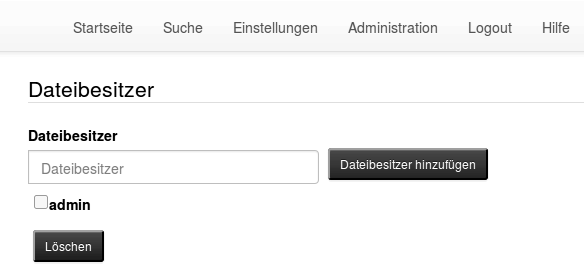
\includegraphics[width=0.9\textwidth]{Masterarbeit_Bilder/einstellungen_dateibesitzer.png}
        \caption{Dateibesitz einem Anwender zuordnen}
        \label{fig:app-cfg-datei}
    \end{figure}  
    
   
    \item Auslesen der Informationen einer Datei unter Beachtung des Dateisystems.
    
    Die Aufgabe wird durch die Java interne API erledigt, dabei wurde für die Attribute eine kleine Abstraktion erstellt, um diese in UTF-8 Kodierung zu schreiben bzw. zu lesen. 
    
       
    \item Anzeigenanpassung und individuelle Unterstützung je nach verwendeter Plattform.
    
    Es wird  der ,,User-Agent'' durch die Weboberfläche ausgelesen, um entsprechende Scripte für die verwendete Plattform zu liefern, wie in Abbildung \ref{fig:app-details} durch ,,open - dir'' oder ,,open - file'' ersichtlich ist.
    Die Anwendung nutzt native Anwendungen wie den Dateimanager zur gewohnter Benutzerunterstützung. Wegen der Limitierungen einer Weboberfläche und den damit verbundenen Sicherheitsbeschränkungen ist die Realisierung von Anwendungen, in denen der Anwendungsbruch kaum spürbar ist, kaum möglich. Für eine bessere visuelle Oberfläche wird auf den Endgeräten eine native Anwendung benötigt und keine Weboberfläche. Die Aufgabenstellung sah dies nicht vor. In der Anwendung ist die Integration daher nur durch Script-Downloads möglich. 
    Sollten die Informationen vom Client nicht richtig sein, wird dem Anwender eine Auswahl von Links, bekannter Plattformen, wie in Abbildung \ref{fig:app-details} gezeigt, aus denen dieser seine Plattform wählen kann.
    
        \begin{figure}[htbp] 
            \centering
            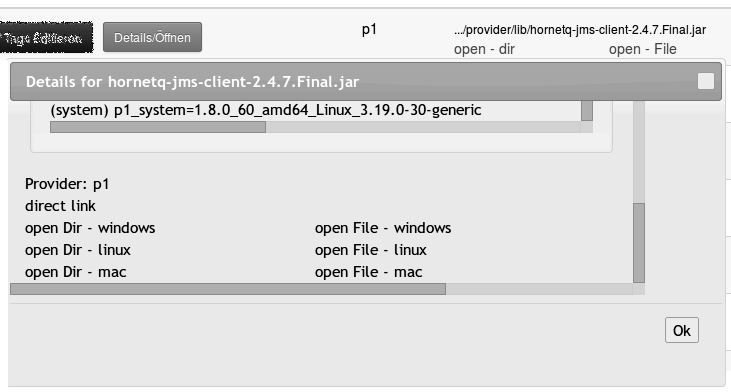
\includegraphics[width=0.8\textwidth]{Masterarbeit_Bilder/details_file.png}
            \caption{Integration in die Plattform, durch Scripte hinter Links}
            \label{fig:app-details}
        \end{figure}  
        
    
    %% ---ralf?
    \item Übertragung der Dateien zwischen teilnehmenden Computern
    
    Diese Aufgabe wird durch Verwendung der ,,externen Befehle'' ermöglicht. Der Mediator vermittelt zwischen den einzelnen Peers die jeweiligen Verbindungsparameter und ermöglicht so einen Dateitransfer. Die Probleme des IPv4 mit \acrshort{nat} wurden nicht durch ,,Connection Reversal'' oder ähnliche Verfahren behoben. Es ist ein Einstellen der Firewall nötig.
    
    \item Benachrichtigung über den Dateizustand
    
     Dateien ohne Schlagworte werden durch periodische Benachrichtigungen dem entsprechenden Anwender als E-Mail gesendet. 
     Mit minimalen Anpassungen können zudem Hinweise zum Kopieren oder Erstellen erfolgen.
     Auch in der Weboberfläche, sofern der Anwender Dateibesitzer ist, sind diese Dateien sichtbar, wie auf dem Ausschnitt der Startseite Abbildung \ref{fig:app-ohnetags} gezeigt.
     
     \begin{figure}[htbp] 
         \centering
         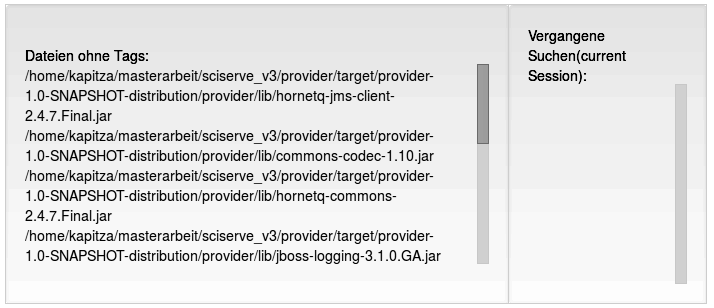
\includegraphics[width=0.8\textwidth]{Masterarbeit_Bilder/ohnetags.png}
         \caption{Dateien ohne Schlagworte}
         \label{fig:app-ohnetags}
        \end{figure}  
        
         
      \item Persistente plattformübergreifende Speicherung der Dateiinformationen
      
      Die Informationen werden in einer eingebetteten Datenbank durch einen Peer gespeichert.
      
    \item Verlinken der \acrshort{dms}
    
    Durch eine ,,bridge'' ist es den Anwendungen möglich, Informationen untereinander auszutauschen. 
    
    \item Erkennung doppelter Dateien
    
    Hier ist keine explizite Anzeige erstellt, doppelte Dateien können dennoch gefunden werden, indem die Prüfsumme in der Suchmaske eingegeben wird. Diese Prüfsumme ist für jeden Dateiinhalt eindeutig, sollte die Datei doppelt existieren, wird das Ergebnis der Suche alle Dateien auflisten. Wie Abbildung \ref{fig:app-dups} zeigt, ist hier die Datei ,,provider-1.0-SNAPSHOT.jar'' in einem Unterordner ,,lib'' vorhanden. Die Prüfsumme wird dabei durch ein ,,\%'' abgekürzt.
    
    \begin{figure}[htbp] 
        \centering
        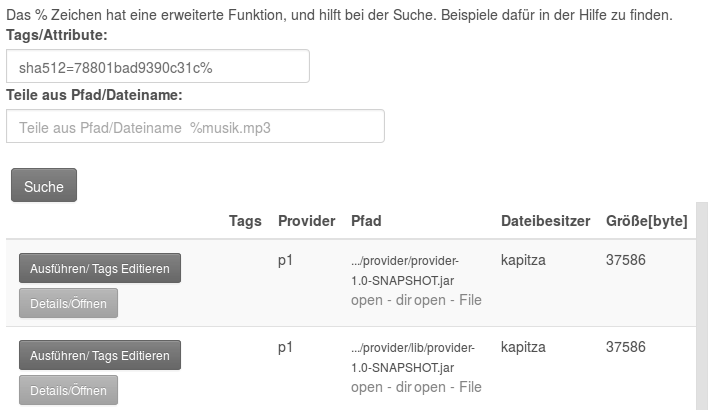
\includegraphics[width=0.9\textwidth]{Masterarbeit_Bilder/suchedups.png}
        \caption{Doppelte Dateien finden durch Prüfsummensuche}
        \label{fig:app-dups}
    \end{figure}  
    
    
    
\end{itemize}



\section{Dateiübertragung}
Dateiverbindungen finden im \acrshort{p2p} direkt zwischen den Peers statt.
Das kann bei IPv4 wegen \acrshort{nat} jedoch schnell zu Problemen führen, da Verbindungen zwischen den Clients je nach Firewall-Typ stark reguliert sind. Der Fall, dass die Peers untereinander nicht die gleichen Protokolle sprechen, ist jedoch selten. Kritisch bleibt je nach Firewall-Typ ein Verbindungsaufbau. In der Abschlussbetrachtung wird auf einige Probleme der Datenübertragung noch einmal gesondert eingegangen und welche Schwierigkeiten sich im Rahmen der Realisierung ergeben haben.

Das Protokoll sieht bereits entsprechende Befehle zum Datenaustausch vor. Dies wird jedoch in der Weboberfläche nur durch die ,,externen''-Befehle nutzbar gemacht (siehe Abbildung \ref{fig:www-cmd-pub}). Durch das Veröffentlichen einer Datei wird im System zwar deren Synchronisieren gestartet, jedoch ist das Steuern der Empfängerpeers nicht möglich.

Durch die Freigabe des Befehls an dem entsprechenden Peer wird dieser angewiesen, seine Daten freizugeben. Ob und wann das Empfangen fertig ist, lässt sich im aktuellen Protokoll jedoch nicht verfolgen. 

\bigskip
Schematisch lässt sich der Ablauf der Dateiübertragung wie folgt beschreiben:

\begin{itemize}
\item Peer A erhält den ,,publish''-Befehl für eine Datei von einem Anwender der Weboberfläche.
\item Peer A sendet Meta-Informationen über die Datei zu allen verbundenen Peers.
\item Jeder Peer prüft selbst, ob er die Datei besitzt.
\\ Wenn: \\
-- Nein: Nachfrage beim anbietenden Peer erzeugen.\\
-- Ja: Kopiert er diese zum angefragten Ziel, sollte diese dort nicht vorhanden sein.\\
\item Jeder nachfragende Peer öffnet einen Port und ermittelt seine externen Verbindungsparameter.
\item Die Verbindungsparameter werden mit Dateiwunsch an alle verbundenen Peers gesendet.
\item Die Peers, welche die Datei besitzen, senden die Informationen zum Nachfragenden.\\
Der Dateitransfer findet direkt zwischen den Peers statt und stört keine weiteren Teilnehmer.
\end{itemize}

In Anlehnung an die in Kapitel \ref{sec:ist} erläuterten Prämissen soll sich die Anwendung einfach in das bestehende Netzwerksystem integrieren. Dazu werden weitere Dienste auf dem Server (vgl. Abbildung \ref{fig:xist-server}) benötigt.
 
Die Endgeräte sind von der Anwendung nicht betroffen. Diese arbeiten wie gewohnt mit ihren Netzwerklaufwerken weiter.
 
\bigskip
 
 \begin{figure}[htbp] 
     \centering 
     \begin{tabular}{|p{.45\textwidth}|}
         \hline
         Server\\ \hline\hline
         ein oder mehrere Dienste wie:\\
         master  | database | provider | www | bridge\\ \hline\hline
         NFS | SMB| Appeltalk | \ldots \\ \hline
         Betriebssystem \\ \hline
         Netzwerk (TCP /IP) \\ \hline
        \end{tabular}
        
        \caption{Server}
        \label{fig:xist-server}
        
    \end{figure}   
    
 
Da es sich um eine \acrshort{p2p}-Lösung handelt, müssen nicht alle Dienste auf jedem Server ausgeführt werden. 
Teile der Anwendung werden von bestimmten Peers bereitgestellt und ergänzen sich zu einer Anwendung, die durch eine Weboberfläche bereitgestellt wird.


In Anlehnung an die ersten \acrshort{p2p}-Netzwerke wie z. B. Napster stellt das ,,master''-Projekt den Kern des Netzwerkes \cite{mahlmann2007peer}.
Dabei kann eine komplexe System-Konfiguration wie in Abbildung \ref{fig:app-outline} aussehen. Es ist natürlich möglich alle ,,Peers'' auf einem Computer oder in virtuellen Maschinen zu installieren.

\begin{figure}[htbp] 
    \centering
    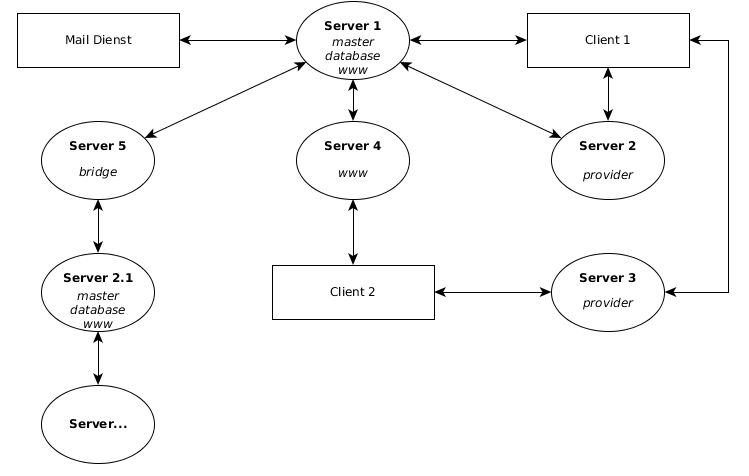
\includegraphics[width=0.8\textwidth]{Masterarbeit_Bilder/clients_uebersicht.png}
    \caption{Übersicht und mögliche komplexere Konfiguration}
    \label{fig:app-outline}
\end{figure}  


 

Hier existieren, neben den diversen Servern, zwei Clients. Die Clients können über die mit einem ,,provider'' versehenen Server Dateisuchanfragen an die ,,database'' stellen.
In der zentralen Datenbank werden die Dateiinformationen gespeichert, um Verschlagwortung und weitere Attribute zu unterstützen.
Ersichtlich ist, dass Lastverteilung durch Erzeugen weiterer Peers einfach zu realisieren ist. 

Datensicherung kann prinzipiell durch eine ,,bridge'' erfolgen. Diese ersetzt aber nicht die Möglichkeit einer im Cluster betriebenen Datenbank und ist damit nicht vergleichbar. Ein Umstellen der Datenbank erfordert lediglich kleine  Anpassungen  in der Konfiguration  der Anwendung ,,database''.


\section{Die Projekte}
Zur Verwaltung der Projekte und deren Abhängigkeiten wird, wie vorab erwähnt, \href{https://maven.apache.org/}{,,Maven''} eingesetzt.
Die Abhängigkeiten der Projekte untereinander ist dabei nicht durch ein  ,,multi module project'' realisiert. Die Verwendung eines  kleines Scriptes auf der Konsole sowie die \acrshort{ide}s lösen diese Problematik auf einfachere Weise. 

Die Kommunikationsschicht wird durch das ,,client'' Projekt bereitgestellt.
Die resultierende Bibliothek muss daher zum Erstellen weiterer Projekte in das lokale Repository installiert werden.
Da der ,,master'',im eingebetteten Modus, zudem von der ,,database''- und dem ,,www''-Projekt abhängig ist, sollten diese zuerst gebaut werden.
Da die Installation der anderen Projekte zu keinen Fehlern führt, genügt das Ausführen von ,,mvn clean install'' in den entsprechenden Projektverzeichnissen zur Erzeugung.

Nachfolgend wird auf die einzelnen Komponenten eingegangen sowie deren Funktionen und Konfigurationen beschreiben.


\subsection{Bridge-Projekt}
Mit dem ,,bridge'' Projekt wird die Idee der Erweiterung des Netzwerkes verfolgt. Wie in Abbildung \ref{fig:app-outline} sichtbar, verbindet dieses Projekt zwei autonome Systeme und ermöglicht einen Informationsfluss über deren Systemgrenzen hinweg. Ein vorteilhafter Nebeneffekt ist das Synchronisieren der Datenbank im laufenden Betrieb.

In komplexen Netzwerkkonfigurationen kann ein Peer mehreren Netzwerken angehören.
Da so mehrfache Antworten auf eine Frage kommen können, müssen die Peers mit Duplikaten und leichten Variationen in den Antworten umgehen können.
Dabei werden die Daten in beide Richtungen der ,,bridge'' gesendet. Diese Dopplungen können durch einen \acrfull{ttl} Wert nicht verhindert werden. Dieser vermeidet lediglich ,,round trips'' innerhalb des Routing.

Die Konfiguration ist einfach gehalten, sie erwartet die ,,master'' IP bzw. \acrfull{fqdn} Adressen sowie ein gemeinsames Geheimnis, um am entsprechendem Netzwerk teilzunehmen.

\bigskip
Beispielsweise lässt sich mit den folgenden Zeilen in der ,,bridge.properties'' eine Verbindung zwischen zwei Systemen herstellen.

\begin{verbatim}
# Eindeutige ID der Bridge in beiden Systemen
de.bluepair.jms.client.id=bridge_host0_host1
de.bluepair.jms.autoconnect=true

de.bluepair.jms.masterkey.0=key1
de.bluepair.jms.ttl.0=1
de.bluepair.jms.host.0=ip1

de.bluepair.jms.masterkey.1=key2
de.bluepair.jms.ttl.1=1
de.bluepair.jms.host.1=ip2
...
\end{verbatim}


\subsection{Provider-Projekt}
Der ,,provider'' stellt Dateiinformationen und Dateien zur Verfügung und reagiert auf Anfragen des ,,master'', zu dem er eine Verbindung aufgebaut hat.
Einem Anwender des ,,www''-Peers ermöglicht er einen konfigurierten Befehl auszuführen. 

Die Kommunikation ist vorrangig vom ,,provider'' nur in Richtung ,,master''. 
Wünsche, welche die Kommunikation unter den Peers beinhalteten, ergaben im Zuge der Entwicklung, dass die Prozessverwaltung in Java ähnliche Probleme wie die Dateiüberwachung aufweist. Diese Wünsche beinhalteten die Befehlsausführung mit externen Programmen aus der Weboberfläche. Viele wünschenswerte Informationen fehlen jedoch in den APIs und konnten dadurch weder am Prozess noch in der Weboberfläche abgebildet werden. Prozesse und deren ID oder OWNER herauszufinden können in Java nur plattformspezifisch realisiert werden und beschränken das Feedback des Prozesses. Ein überwachen, bei lang andauernden Hintergrundaufgaben, ist in der Anwendung daher nicht möglich. Es ist auch hier nötig, eine Fassade über das von Java bereitgestellte Prozessverwaltungssystem zu entwickeln.

Die ,,externen'' Befehle ermöglichen zudem API interne Aufrufe wie ,,publish'' Anwendern freizugeben.
Deren Argumente sind im Unterschied zu ,,externen''-Befehlen durch die Anwendung fest vorgegeben. 

\bigskip
In der Konfigurationsdatei ,,provider.properties'' können Befehle einfach angemeldet werden.

\begin{itemize}
    \item Der interne Befehl ,,publish'' kann für die ,,www''-Anwendung freigegeben werden.
    (Andere werden derzeit nicht unterstützt da sich diese nicht für Anwender eignen.)\\
    \verb|publish.internal=true|
    
    \item Der externe Systembefehl ,,cat'' unter Linux wird durch zwei Einträge freigegeben. Einmal muss der Befehl als solcher definiert werden während dessen Argumente, die meist anderen Regeln folgen, in der ,,www''-Anwendung mit Platzhaltern vorbelegt werden. Hier ist der Platzhalter ,,\{\}'' konfiguriert. Da  diese Sonderzeichen in Java eine spezielle Bedeutung haben, müssen die Zeichen geeignet maskiert werden.
    \\
    \verb|cat.path=/bin/cat|\\
    \verb|cat.replacewithpath=\\{\\}|
    
\end{itemize}

 

In der Konfigurationsdatei finden sich weitere optionale Parameter. Neben den Standardparametern wie \acrshort{fqdn} bzw. IP sind folgende Werte erlaubt:\\

\begin{itemize}
    \item Zeit in Millisekunden, die vom Watchservice gewartet werden, bevor ein Event stattfindet. Hier wird der Wert auf eine Sekunde gesetzt.\\ \verb|de.bluepair.watchservice.polling=1000|

\item In Linux können Duplikate in den Events durch Angeben von dem Wert ,,true'' verhindert werden. \\
\verb|de.bluepair.watchservice.nodupes=false|

\item Das Programm benötigt Schreibrechte auf den Dateien, auf denen es die  Prüfsumme berechnet. Mit ,,true'' wird ein ständiges Neuberechnen erzwungen, selbst wenn keine Berechtigung zum Schreiben vorliegt.\\
\verb|de.bluepair.watchservice.readonly.force=false|

\item Einige Befehle haben eine erzwingende Option.
Mit ,,true'' kann dieses Verhalten vermieden werden, wodurch ein Überschreiben von Dateien verhindert wird. Diese Angabe hat bei der Nutzung von externen Befehlen und Vorverarbeitungen  keinen Effekt.\\
\verb|de.bluepair.nodelete=true|

\item Wird kein Port für den Dateitransfer angegeben, wählt die Anwendung durch das Betriebssystem einen beliebigen freien Port. Das Konfigurieren einer Firewall ist ohne konkreten Port schwer. Für Windows ist empfohlen einen Port festzulegen.\\
\verb|de.bluepair.provider.fileget.port=6666|
\end{itemize}

\subsection{Client-Projektbibliothek}

Das ,,client'' Projekt ist eine Bibliothek, die von Peers verwendet wird, um eine einheitliche Kommunikation zu gewährleisten. Es stellt eine API bereit, um einfach mit \acrshort{jms} zu agieren.

Zudem kommt die oben erwähnte Abstraktion des Watchservice, auf dessen Realisierung hier eingegangen wird, was Peers ein gezielteres Arbeiten mit Dateievents erlaubt.

Zu den in jeder ,,PROJEKT.properties'' anzutreffenden Konfigurationen gehören:

\begin{itemize}
    \item
    Diese Einstellung lässt im Fehlerfall des Peers einen erneuten Verbindungsaufbau stattfinden.\\
    \verb|de.bluepair.jms.autoconnect=true|
    
    \item Die Kommunikation unter den Peers wird durch ein gemeinsames Geheimnis gesichert. Dieses wird i. d. R. vom ,,master'' festgelegt. Das Geheimnis stellt bei  Vermittlung sicher, dass keine unerwünschte Nachricht weitergeleitet wird.\\  
    \verb|de.bluepair.jms.masterkey=sharedKey|
    
    \item Die Verbindung zum Vermittler erfolgt über den Host Eintrag.
    Dieser stellt \acrshort{jms}- und \acrshort{stun}-Dienste, für evtl. weitere andere Direktverbindungen, bereit.\\
    \verb|de.bluepair.jms.host=IP_OR_FQDN|
    \item Jeder Client sollte im Netzwerk einen eindeutigen Namen haben. Es ist kein \acrshort{fqdn} nötig, jedoch bei großen Netzen zu empfehlen. Dieser Eintrag wird z. B. bei ,,www'' verwendet, um weitere Konfigurationen eines ,,provider'' einzustellen.\\
  \verb|de.bluepair.jms.client.id=UNIQUE_ID|
\end{itemize}


\subsubsection{Java NIO}
Das Java ,,new/non-blocking Input Output'' API ermöglicht Java Anwendungen seit Version 7 einen ,,WatchService'' zu verwenden. Dieser Service kann zur Ordnerüberwachung eingesetzt werden. Dabei werden ,,polling'' und ,,interrupt'' Ansätze unterstützt.

Leider wird von diesem Service bei einer Dateiänderung nur der Dateipfad zur Datei, nicht aber Auskunft über den Prozess, übertragen. Auch bei den Events mangelt es an fehlender Informationen. Die Ereignisse CREATE, DELETE, MODIFY reichen für das Arbeiten mit wissenschaftlichen Daten nicht aus. Ein ständiges Überprüfen, ob es sich um ein noch aktives Kopieren handelt, verschwendet Ressourcen. Eine neue Datei wird, wenn sie durch eine längere Kopieraktion entsteht, mehrmals das Event MODIFY durchlaufen. Wird dieses Event zum Anlass genommen für Berechnungen, würden diese häufig gestartet und abgebrochen werden.  Ein ONCOPY-Event wäre für die Verarbeitung einer solchen Datei einfacher zu verwenden und könnte durch ein FINISH-Event als beendet markiert werden. So lassen sich ständige unnötige Neuberechnungen auf Dateiinhalte vermeiden.

Eine Fassade  über dem ,,WatchService'' sieht daher mehr als die in  ,,StandardWatchEventKinds'' bestehenden Events vor \cite{gamma2011entwurfsmuster}. So werden Events von der Fassade aggregiert und nur etwa alle 5 Sekunden weitergegeben. Eine abweichende Zeit lässt sich beispielsweise im ,,provider'' einstellen. Dabei werden bei Events auf dem gleichen Dateipfad folgende Regeln beachtet.

\begin{itemize}
    \item Auftreten von zwei MODIYFY Events \\
    löst ein ONCOPY und ein MODIFY Event aus.
    \item Auftreten von zwei ONCOPY Events\\
    löst nur ein ONCOPY Event aus.
    \item Auftreten vom letzten MODIFY Event nach Starten des ONCOPY\\
    löst ein FINISH Event im nächsten Zyklus aus.
\end{itemize}

Dadurch wird das Verwenden der Überwachung flexibler und das Unterdrücken anhand der Regeln, von einigen Events, wird durch ,,addSuppressed'' und ,,getSuppressed'' mit Exception-Behandlung vergleichbar, wodurch bei Bedarf mehr Details zum Event abgefragt werden können.

%% --ralf?
Die Fassade kann der Problematik, den Änderungsprozesses zu erkennen, nicht zuverlässig entgegen kommen und liefert die Informationen daher nicht mit. Das Auslesen von Betriebssystemprozessen ist nicht trivial lösbar. Dieses Problem tritt innerhalb der Anwendung auch bei den ,,externen'' Prozessen auf.

Anders als der ,,WatchService'' gibt die Fassade den absoluten Pfad weiter, da sich damit einfacher arbeiten lässt als mit einer relativen Angabe zu einem zum Triggerzeitpunkt ,,unbekannten'' Ordner.

Auch das Arbeiten mit erweiterten Attributen konnte so vereinfacht werden.
Durch ein entsprechendes Event werden alle nötigen Operationen, um Attribute lesen oder schreiben zu können, bereits vom Event bereitgestellt. Das Arbeiten mit diesem Event entspricht daher einer Fusion verschiedener Java-API wie ,,WatchEvent'', ,,Path'', ,,Files'' und ,,File''.

Es ergeben sich Nachteile bei der Verwendung  der Fassade. Events sind nicht mehr in Echtzeit übertragbar, da eine Verzögerung vor der Weitergabe entsteht. Dies steht aber mit den hier genannten Daten in keinem Konflikt. Durch das Veralten der Events ist ein Weiterarbeiten nicht mehr nötig oder möglich. Beispielsweise ist ein Kopiervorgang mit anschließendem direkten Löschen ein möglicher Kandidat für Fehler, sowie das Weitergeben eines MODIFY-Event bei dem keine Datei mehr zugrunde liegt.
Der Problematik wird durch Prüfung der Dateievents vor der Weitergabe entgegengewirkt.

\bigskip
Dabei treten speziell die Konflikte auf:

\begin{itemize}
    \item MODIFY zu DELETE \\
    Wie oben erwähnt, kann eine Dateiänderung mit anschließendem Löschen die Änderung gänzlich eliminieren, da die Änderungen nicht mit übertragen werden.
    \item CREATE zu DELETE \\
    wegen Transitivität (CREATE -> MODIFY -> DELETE) verhält sich dieser Fall wie oben beschrieben.
\end{itemize}

Die Verwendung der Fassade, zum Berechnen von Prüfsummen, muss nicht sicherstellen, dass jede Änderung berücksichtigt wird.
Änderungskonflikte durch ersetzendes Kopieren von Dateien werden daher nicht gesondert betrachtet.

Die Fassade selbst realisiert ein Beobachter-Muster, um ihre Dienste anzubieten \cite{gamma2011entwurfsmuster}.

Als Kommunikationsextra ist es möglich, der Fassade Events zu injizieren. So muss nicht zwangsweise eine Änderung auf dem Dateisystem stattfinden.

Dies wird mit einem UPDATE Event realisiert.
Dabei steht dieses in Konflikt mit allen anderen Events und soll sicherstellen, dass in jedem Fall mindestens ein Event im nächsten Ausgabetakt stattfindet.

Um Extra-Informationen an ein Event anzuhängen, wurden Events, wie bei den meisten Controls von JavaFX, mit den Methoden ,,getUserData'' und ,,setUserData'' erweitert. Dadurch lassen sich beliebige Objekte durch die Anwendung transportieren. 



\subsubsection{Java Mail}
Die Java-Mail-API wurde verwendet, um einen schnelleren Zugriff auf E-Mails zu erhalten. Dabei wurde die API so implementiert, dass diese mit den Funktionen aus Java 8 verwendet werden kann.

Eingehende E-Mails sind in dieser API nicht mehr vom Mail-Server getrennt und können direkt Antworten generieren und versenden. Das vermeidet unnötig viele Referenzen auf Objekte und erlaubt bei Verwendung ein einfacheres Arbeiten.

Die API muss im Internet seit April 2014 eine Verschlüsselung verwenden, um mit den gängigen anderen Mail-Servern zu kommunizieren \cite{sslmail}. Daher sind für die API weitere Konfigurationsparameter erforderlich.
\label{javamailc}
\begin{itemize}
    \item Zu den Standardparametern gehören die Verbindungsparameter zum Server.\\
    \verb|de.bluepair.mail.port=SMTP_PORT|\\
    \verb|de.bluepair.mail.host=IP_OR_FQDN|\\
    \verb|de.bluepair.mail.user=USER|\\ \verb|de.bluepair.mail.password=USER_PASSWORD| - das Passwort ist in Klartext anzugeben und wird für IMAP und SMTP verwendet. \\
    \verb|de.bluepair.mail.address=USER@FQDN| - die Sender-Adresse unter der E-Mails versendet werden. 
    \item Aus der Java-Mail-API können beliebige Parameter  durch Verwendung eines PREFIX \verb|de.bluepair.| aufgenommen werden.
    \verb|de.bluepair.mail.smtp.ssl.trust=*| und\\
    \verb|de.bluepair.mail.imap.ssl.trust=*| werden standardmäßig gesetzt.
    
\end{itemize}

Wegen der verwendeten Testumgebung und der oben genannten Problematik, dass eine Verschlüsselung zwingend notwendig ist, sind die \verb|ssl.trust| Parameter standardmäßig auf ,,*'' gesetzt. Dies umgeht einige Schutzfunktionen der zertifikatbasierten Kommunikation, es ist ratsam diese Parameter an die Einsatzumgebung anzupassen und gegebenenfalls eine ,,socketFactory'' zu implementieren. 

\subsection{Database-Projekt}
Das ,,database''-Projekt stellt die Kernfunktionalität für die Suchen und dem versenden von Benachrichtigungen bereit.
Das betrifft bei der Speicherung der zusätzlichen Dateiinformationen eine entsprechende Verwaltung der Daten in einer SQL-Datenbank.
Die Anwendung kann dabei mit eingebetteten Datenbanken oder extern wie z. B. {MySQL} oder {PostgreSQL} betrieben werden.
Wegen der Nutzung von \acrshort{jpa} sind innerhalb der Anwendung keine Anpassung nötig, da SQL-Anfragen entsprechend dem Treiber der Datenbank erzeugt werden.
Die Abbildung der Tabellen auf Java-Objekte ist überschaubar und verfolgte einen ,,Code-First'' Ansatz (vgl. \cite{wincodefirst}). 

Durch den Anwendungsserver ist eine Konfiguration wegen der Zentralisierung sehr einfach gehalten. Durch einen \acrfull{acc} wäre das Realisieren eines Peers möglich, jedoch ist dieser wegen des verwendeten Anwendungsserver zu Fehlerhaft. Die Problematik, dass im eingebetteten Modus nicht alle Konfigurationen zu Verfügung gestellt werden, erschwert das Verwenden des \acrshort{acc} zudem und bietet keinen Mehrwert in der Funktionalität für die Anwendung.

Bei der Auswahl einer Datenbank muss lediglich darauf geachtet werden, dass dessen Treiber JDBC unterstützen. 
Die Verwendung von \acrshort{jpa} ist zwar langsamer als das Schreiben von entsprechenden SQL-Anweisungen, der Vorteil liegt aber in der konsequenten Vermeidung von SQL-Injektion und direkten Nutzen von Objekten.


Alle Nachrichten, die am ,,master'' eingehen, werden von diesem an die Datenbank weitergeleitet und dort verarbeitet. Dadurch kann neben der reinen Speicherung eine Statistik erhoben werden. Das Benachrichtigungssystem, welches in diesem Peer realisiert ist, versendet Erinnerungen anhand des Datenbestandes und versucht mit diesen den Anwender zu ermuntern, den Datenbestand zu verbessern.
Die dazu erzeugte E-Mail wird jedem registrierten Anwender durch die hinterlegte E-Mail-Adresse gesendet.

Das System berücksichtigt dabei die Einstellungen des Anwender durch die Option \verb|email.push=true|, und versucht die Adresse entweder aus dem Login oder entsprechender Option \verb|email=MAIL@FQDN| zu erkennen.

Um die Häufigkeit der Benachrichtigungen zu steuern, können in der Konfiguration neben den oben genannten Java-Mail-Einstellungen (\ref{javamailc}) die Zeitintervalle zum Versenden und Bearbeiten von E-Mails eingestellt werden.

\begin{itemize}
    \item Die Überwachung eines IMAP-Ordner muss dazu angegeben werden.\\
    \verb|de.bluepair.mail.mailbox=INBOX| - INBOX ist i.d.r. Standard
    \item Anschließend kann das E-Mail Verarbeitungsintervall wie unten auf z. B. eine Sekunde eingestellt werden.\\
    \verb|de.bluepair.mail.imap.polling=1000|
    \item Das Erinnern via E-Mail kann unabhängig von der Verarbeitung festgelegt werden. Die hier erteilten 10 Sekunden sind nicht in der Produktion zu empfehlen, da dadurch gerade zur Einführungsphase eine erhebliche Menge an E-Mails versendet werden könnten.\\
    \verb|de.bluepair.mail.reminder=10000|
    \item Bei der Erzeugung von E-Mails wird ein Link für die Weboberfläche generiert. Für einen richtigen Link wird der Port benötigt. Standardmäßig wird der Port 8080 verwendet. Ein anderer wird durch \\
    \verb|de.bluepair.www.port=7070| angegeben. Als Host wird der Eintrag \\
    \verb|de.bluepair.www.host=FQDN| verwendet und bei keiner Angabe \\
     \verb|de.bluepair.jms.host=FQDN| der ,,master'' angenommen.
    
    \item Angaben für den einfachen \acrshort{stun} Dienst erfolgen mit \\
    \verb|de.bluepair.jms.echo.port=8888|
    
\end{itemize}
 
Dieser Peer nutzt zur Verarbeitung anders als alle bisherigen Peers eine Bibliothek für \acrshort{cdi} und Events. 
Das Verarbeiten von den eingehenden Nachrichten läuft dabei mehrstufig ab und nutzt ein Layer Architekturmuster \cite{buschmann1998pattern}.

Neue Dateien werden vor dem Speichern in der Datenbank auf ähnliche, bereits vorhandene, Einträge untersucht.
Aktuell hilft dabei die Prüfsumme, so dass Tags, die von Anwendern vergeben wurden, direkt für neue Dateien gelten. Das vermeidet unnötige Erinnerungen für Dateiduplikate  zu versenden.

Handelt es sich um ,,Datei fremde'' Nachrichten, wie Anfragen vom ,,www''-Peer, stellt die Anwendung eine einfache Benutzerverwaltung, die neben der üblichen Funktionen  einem oder mehreren Anwendern Dateien zuordnen kann.

Die verwendete eingebettete Datenbank erzeugt sich komplett selbst, die Konfigurationen dieser können nicht ohne Sourcecode Anpassungen getätigt werden.
Das Abstellen und Einrichten neuer Verbindungsparameter zu anderen Datenbanken erfordert daher grundlegende Programmiererfahrungen mit der \acrshort{jpa}.



\subsubsection{Mail Service}
Da bereits vorab auf die Konfiguration der E-Mail-Funktion eingegangen wurde, wird hier nur noch der Mehrwert für den Anwender beschrieben.

Die vom System versendete E-Mail ist so präpariert, dass ein Anwender durch Antworten auf diese E-Mail dem System Schlagworte zur Datei mitteilen kann.

Dazu darf der E-Mail-Inhalt nicht gelöscht werden, wichtig ist hier die Prüfsumme zu erhalten. Das System reagiert auf das Schlagwort \verb|TAGS=|, welches in der E-Mail verwendet werden soll, um Schlagworte der entsprechenden Datei zuzuordnen.



\subsection{Master-Projekt}

Der ,,master''-Peer stellt als eingebettete Version die größte  Funktionalität. Zu diesen zählt das Vermitteln von Nachrichten, um den Peers die Kommunikation zu ermöglichen. Beim Dateiaustausch der Peers übernimmt der Vermittler eine zentrale Rolle und vermittelt die Ports und Adressen zwischen den Teilnehmern (vgl. FTP-Protokoll \cite{rfc959}).


Auch ein primitives \acrshort{stun} ist implementiert, um IP und Port eines Peers zu erkennen. Jedoch beschäftigt sich diese Arbeit nicht mit der Problematik des ,,Hole Punching'' und geht davon aus, dass Firewalls zwischen den Peers die Kommunikation erlauben.


Dieser Peer prüft die Kommunikation zwischen Peers, sofern diese untereinander reden wollen, auf den von ihm vergebenen gemeinsamen Schlüssel.
Die zwei verwendeten Kommunikationskanäle unterscheiden sich in der Verlässlichkeit des Nachrichtentransports. 
Nachrichten an diesen Peer werden durch ein ,,Queue'' geregelt. Diese speichert die Nachrichten im Fall der Abwesenheit zwischen. Die Kommunikation der Peers wird durch eine ,,publish-subscrib''-Architektur ermöglicht. Sie erlaubt eine effiziente nicht zuverlässige Kommunikation zu allen Peers. Die Problematik wird durch Verwendung von TCP auf An- und Abwesenheit eines Peers eingeschränkt, da nur Einwegnachrichten verwendet und TCP-Nachrichten nur ganz oder nie übertragen werden. 

Die direkte Kommunikation zwischen den Peers beschränkt sich aktuell auf den Dateitransfer. Der generelle Nachrichtenaustausch ist an ,,Napster'' angelehnt und läuft immer über den Vermittler.


Im eingebetteten Modus werden alle nötigen Dienste gestartet. Dabei wird die Konfiguration auf das nötigste beschränkt. Zu den eingebetteten Diensten gehören das \acrshort{jms}, ,,database'', ,,www'' und ein Anwendungsserver. Nachfolgend wird auf die speziellen Parameter für diesen Peer eingegangen, generelle Parameter der Anwendung können den entsprechenden Kapiteln entnommen werden.

\begin{itemize}
    
    \item 
    Ist dieser Parameter nicht angegeben, wird dieser automatisch erzeugt. Er kann in der kleinen Shell, nach Anwendungsstart, durch den Befehl ,,masterkey'' oder der entsprechenden Konfigurationsdatei nachgesehen werden.\\
    \verb|de.bluepair.jms.masterkey=SHARED_KEY|
    \item Der Webserver kann auf einem beliebigen Port gestartet werden. Damit kein Konflikt entsteht, wird per Standard \verb|7070| verwendet. Das wird in der Konfiguration mit \\
    \verb|jsf.port=7070| angegeben. \\
    Webanwendungen können durch den ,,deploy''-Befehl und der Angabe von Datei, Name und Kontext als Parameter installiert werden, sowie durch ,,undeploy'' und Angabe des Namen zerstört werden.
    Für die Basisanwendung werden alle Kontexte überschrieben, es ist ein Neukonfigurieren nötig, um andere Anwendungen zu erlauben. Für die Basisanwendung wird automatisch der Befehl\\
    \begin{quote}
        deploy www.war www /
    \end{quote}
     abgesetzt. Dies kann durch die Angabe von ,,false'' im Parameter\\
     \verb|de.bluepair.www = true| verhindert werden.\\ Einen anderen Dateinamen kann man durch \\
     \verb|de.bluepair.www.file = www.war| festlegen. Dabei wird vom Ausführungsort anfangend nach dieser Dateiangabe gesucht.
     
     \item Die Integration des ,,datenbank''-Peer in den ,,master'' und dessen automatisches Starten kann hier ähnlich abgestellt werden. Der Parameter hierfür lautet \\
     \verb|de.bluepair.database = true|
     
     
     \item Die interne einfache \acrshort{stun}-Implementierung kann als Dienst durch \\
     \verb|ipecho.port=8888| auf einen beliebigen anderen Port verschoben werden. Andere Angaben als der Standardport, müssen in den Clients angepasst werden.
      
     
    
\end{itemize}


Es gibt noch einige kleinere Befehle für die Shell, was das Debuggen vereinfachen kann. Dazu gehören ,,property KEY VALUE'', um eine neue Umgebungsvariable ,,KEY'' auf den Wert ,,VALUE'' zu setzen, und ,,send ...'', welches eine mit Leerzeichen getrennte Wortliste annimmt, um Nachrichten in das \acrshort{p2p}-Netzwerk zu senden. Der ,,print'' Befehl ermöglicht Nachrichten auf der Konsole ausgeben und dient der Fehlersuche.

Um wichtige Kommunikation wie das Vernetzen der ,,master'' und das Speichern getrennt zu halten, wurden weitere Kanäle  für die ,,bridge'' und ,,database'' eingeführt. Diese sind als eine ,,publish-subscrib''-Architektur entworfen. Der Unterschied zum bestehenden Kommunikationskanal ist das Entfallen der Prüfung des gemeinsamen Geheimnisses.



\subsection{Weboberfläche}
In dem Unterprojekt ,,www'' wird die Interaktion mit dem Anwender durch eine in HTML erzeugte Oberfläche realisiert.
Das Suchen erfolgt in der \acrshort{p2p}-Netzwerkdatenbank der speichernden Peers, welche zudem Konfigurationen und eine primitive Benutzerverwaltung bereitstellen.
Ein angemeldeter Anwender erhält mehr Möglichkeiten für die Interaktion mit den einzelnen Peers. Dazu zählen beispielsweise das Filtern von Dateien durch externe Prozesse, das Eintragen und Editieren von Tags und das Konfigurieren von den Pfaden zu Netzlaufwerken auf der eigenen Festplatte über ,,reguläre Ausdrücke''.

Da die Konfiguration nicht durch eine Properties-Datei realisiert werden kann, müssen die Einstellungen am Anwendungsserver erledigt werden. Für den eingebetteten Modus reicht die Konfigurationsdatei des ,,master''. Beim externen Betreiben ist es nötig, die wichtigsten \acrshort{jms}-Parameter durch Umgebungsvariablen zu definieren. Das kann global im System oder -- je nach Anwendungsserver -- für die Anwendung separat gemacht werden.

Auf die Möglichkeiten eines Anwender zur Interaktion wird nachfolgend eingegangen.
Dabei wird sich an den oben genannten Szenarien gehalten. Diese waren:

\begin{itemize}
    \item Das Dateisuchen.
    \item Der Dateizugriff.
    \item Die Dateisynchronisation.
\end{itemize}

In der folgenden detaillierteren Betrachtung werden globale Strukturen, Navigationshinweise und Konfigurationen der Anwendung ohne Wiederholung betrachtet. 
Es wird in den einzelnen Szenarien nur ein Ausschnitt betrachtet, welche den in der Abschlussbetrachtung besprochenen Versuchsaufbau nutzen.

Durch die Verwendung von HTTP-Sessions muss grundsätzlich bei längere Inaktivität mit Datenverlust gerechnet werden, da durch eine ablaufende Session, die vergleichbar mit einem Abmelden vom System ist, alle nicht gespeicherten Daten verloren gehen.
Dateispeicherungen und das Editieren von Formularen sollte daher zügig erledigt werden. Mit Session-Start, welcher durch erstmaliges Betreten der Anwendung erfolgt,  wird der Anwender automatisch auf die Startseite (Abbildung \ref{fig:www-start}) umgeleitet. Durch das Abmelden, bei zu langer Inaktivität oder durch Klicken wird eine neue Session gestartet. Auf dies wird mit einem Umleiten auf die Startseite reagiert.


\begin{figure}[htbp] 
    \centering
    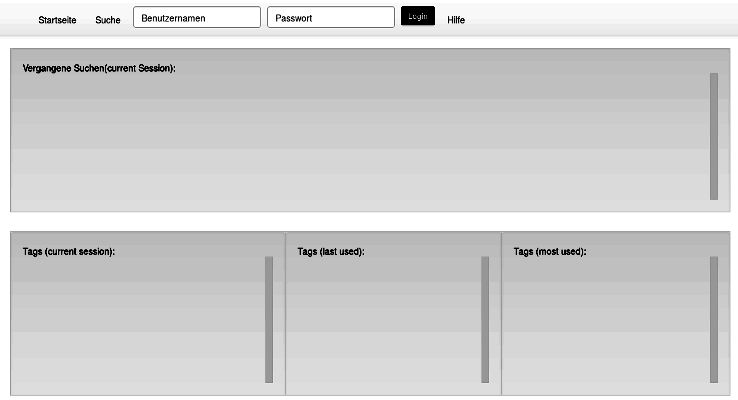
\includegraphics[width=\textwidth]{Masterarbeit_Bilder/www_startseite.png}
    \caption{Startseite der Webanwendung}
    \label{fig:www-start}
\end{figure}  



\begin{figure}[htbp] 
    \centering
    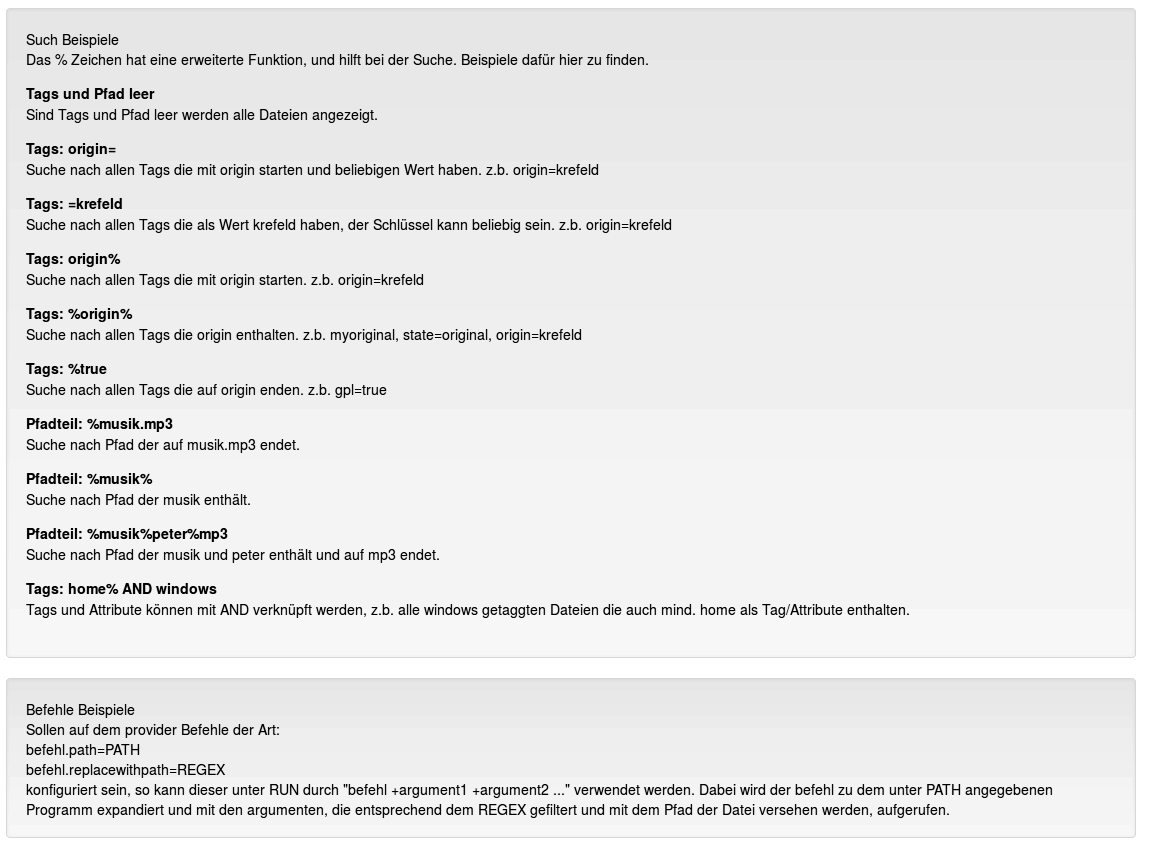
\includegraphics[width=0.8\textwidth]{Masterarbeit_Bilder/www_help.png}
    \caption{Hilfeseite}
    \label{fig:www-help}
\end{figure}  




Es wird kein ,,Faces Flow'' verwendet. Bei Session-Inaktivität wird der auftretende Fehler durch eine konfigurierte Umleitung abgefangen. Ist das Nutzerverhalten evaluiert und fest, ist eine Verwendung der ,,Faces Flow''-API sinnvoller.

Die Abbildung  \ref{fig:www-start} zeigt zudem oben rechts die ,,Hilfe'' an. Auf diese wird innerhalb der Anwendung öfter verwiesen. Hier stehen Beispiele und Erklärungen wie Abbildung \ref{fig:www-help} zeigt. 
%% ab hier gehts weiter!!
Da erst nach dem Einloggen alle Funktionen nutzbar sind, sollte der Anwender oben rechts (vgl. Abbildung \ref{fig:www-start}) seinen Benutzernamen und ein Passwort eintragen.
Für den ersten Login werden Administrator-Rechte vergeben. Alle weiteren neuen Anwender bekommen anschließend nur durch diesen Administrator weitere Rechte. Sollte ein Anwender sich das erste Mal am System anmelden, wird automatisch ein Konto angelegt. Sollte das Konto existieren, werden die Identifikationsdaten überprüft und der Anwender bei Erfolg eingeloggt.
Anschließend stehen ihm Konfigurationen und im Fall des Administrators administrative Optionen zur Verfügung.
Die Abbildung \ref{fig:www-einstellungen-admin} zeigt einen eingeloggten Administrator mit leeren Einstellungen und Abbildung \ref{fig:www-einstellungen-user} mögliche Benutzereinstellungen.



\begin{figure}[htbp] 
    \centering
    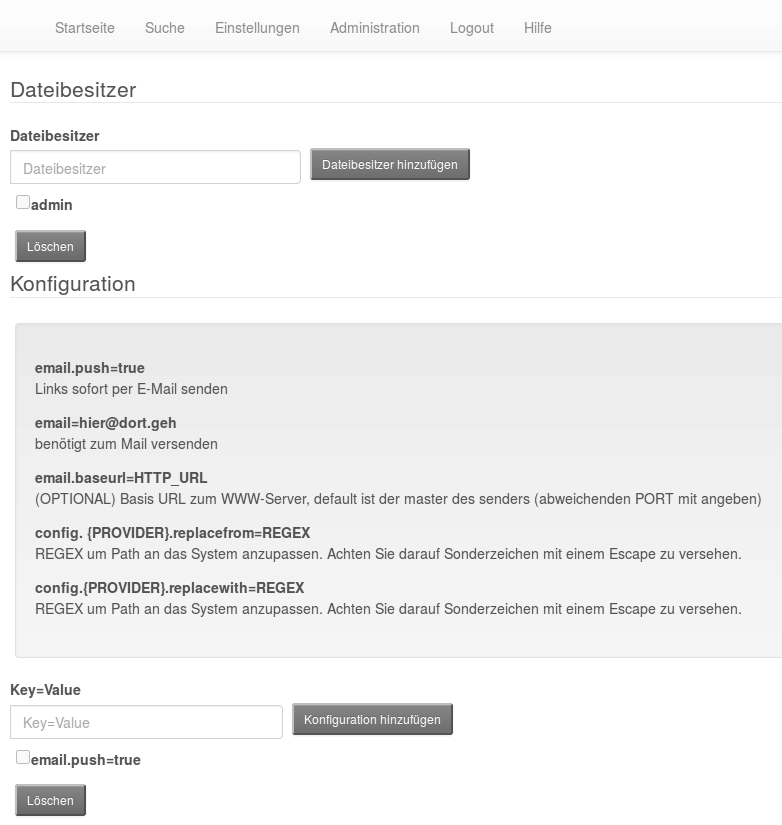
\includegraphics[width=\textwidth]{Masterarbeit_Bilder/www_einstellungen_user.png}
    \caption{Einstellungen eines Anwenders}
    \label{fig:www-einstellungen-user}
\end{figure}  



\begin{figure}[htbp] 
    \centering
    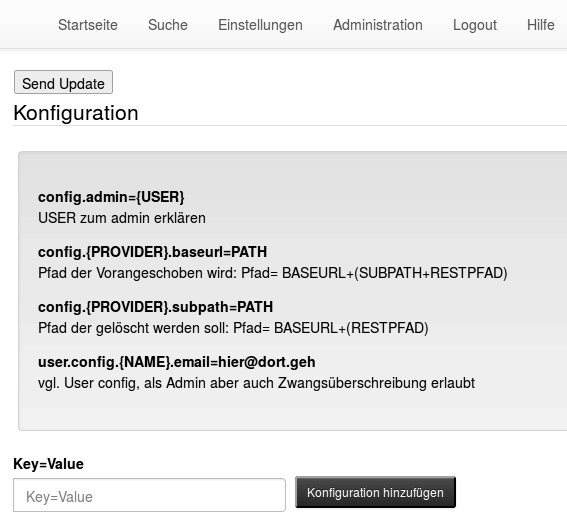
\includegraphics[width=\textwidth]{Masterarbeit_Bilder/www_einstellungen_admin.png}
    \caption{Einstellungen des Administrator}
    \label{fig:www-einstellungen-admin}
\end{figure}  



Nachfolgend gehen alle Szenarien auf die Suche ein, durch einen Klick auf ,,Suchen'' kann dorthin navigiert werden. 



\subsubsection{Suche über den Datenbestand}
Die Suchmaske enthält  zwei Eingabefelder, einen Button und eine Ergebnisauflistung, wie in Abbildung \ref{fig:www-suche} zu sehen ist.
Die in der Analyse angesprochenen Probleme, wie die Plattform übergreifende persistente Speicherung der Schlagworte, ist hier durch Nutzung einer dezentralen Datenspeicherung gelöst. Nutzer verschiedener Plattformen bekommen  für ihre Suche immer die gleiche Oberfläche präsentiert. Um der Plattformunabhängigkeit gerecht zu werden, weichen die Abfragesprache und die Ergebnisauflistung zwischen diesen nicht ab. Die Datenbank legt alle Daten als Zeichenketten ab und beschränkt damit die Suchen auf Mustervergleiche. Diese lässt sich später erweitern und könnte mehr Unterstützung von Vergleichsoperatoren, wie größer oder kleiner sowie ,,Boolesches Retrieval'' bieten \cite{kuhlen2013grundlagen}. Nachfolgende Beispiele beschränken sich allerdings auf Mustervergleiche und erlauben eine Suche nach Dateinamen und eine Suche nach Attributen wie ,,mime-type'' oder ,,Erstellungsdatum''.
Werden Dateipfade und Attribute gleichzeitig gesucht, wie in Abbildung \ref{fig:www-suche2} zu sehen, werden diese durch ein ,,UND'' auf der Datenbank verbunden.



\begin{figure}[htbp] 
    \centering
    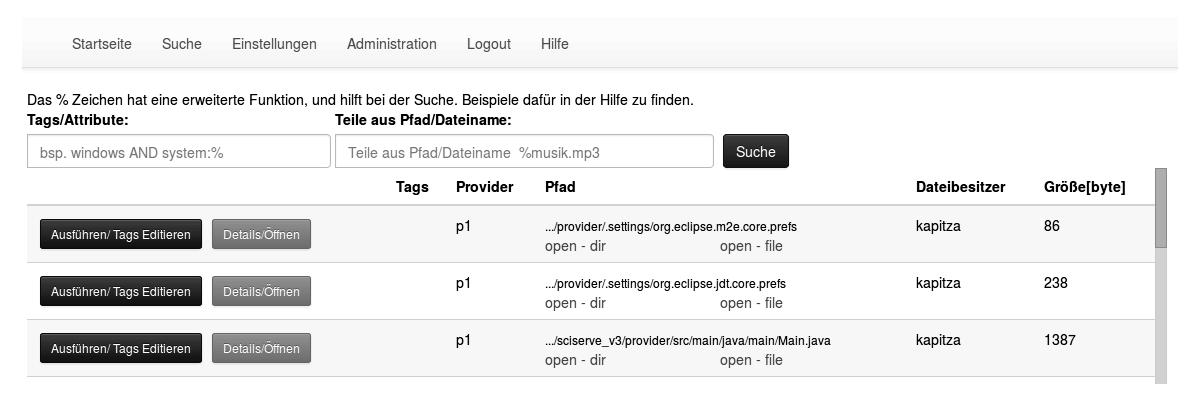
\includegraphics[width=\textwidth]{Masterarbeit_Bilder/www_suche.png}
    \caption{Suchfenster mit leerer Beispielanfrage}
    \label{fig:www-suche}
\end{figure}  

\begin{figure}[htbp] 
    \centering
    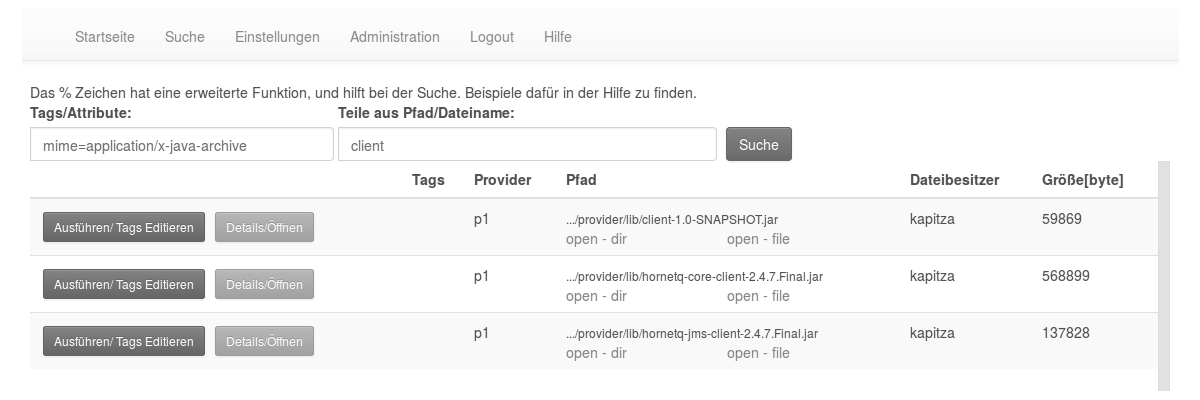
\includegraphics[width=\textwidth]{Masterarbeit_Bilder/www_suche2.png}
    \caption{Suchfenster mit Beispielanfrage nach ,,JAR'' Datei mit ,,client'' im Dateipfad}
    \label{fig:www-suche2}
\end{figure}  

 
\subsubsection{Zugriff auf den Datenbestand}
In diesem Szenario wird gezeigt, wie die Anwendung dem Anwender hilft, auf die im Netzwerk abgelegten Daten zuzugreifen. Wegen der Limitierungen durch den Webbrowser, bedingt durch Sicherheit und nutzbare Funktionen, findet keine Übertragung der Daten statt und eine direkte Integration in den Desktop ist nur durch Umwege möglich.
Dennoch erfolgt der Dateizugriff für den Anwender  durch einen vom Betriebssystem bereitgestellten Dateimanager. 
Dazu erkennt die Anwendung anhand des ,,User-Agent'' das Betriebssystem des Anwenders und generiert für dieses ein passendes Script. Dies setzt voraus, dass der Anwender die Netzwerklaufwerke bereits konfiguriert hat.

Um das Anpassen und Integrieren in den Desktop zu erklären, wird Ein ,,provider'', beispielsweise mit eindeutigem Namen ,,wichtigedaten'' auf dem Computer ,,server1'' angenommen. Dieser übermittelt alle Meta-Informationen an die Datenbank, nach denen der Anwender suchen kann. Nun kann ein Administrator Standardeinstellungen zum ,,provider'' festlegen. Diese Einstellungen beschreiben die Abbildung der Festplatte des ,,provider'', von der die Daten mit absoluten Pfad kommen, zu deren Abbildung auf eine Netzwerkfreigabe.


Anschließende Bilder beziehen sich auf ein Linux System. Die Beschreibungen der Anwendung sind am Beispiel Windows, um zumindest zwei Plattformen beispielhaft zu Zeigen.
Die Bilder nutzen die Konfiguration, wie diese in der Abschlussbetrachtung durch die Testumgebung vorgestellt ist. Als Basis wird dort der Pfad ,,/opt/files'' auf dem Server und ,,/data'' auf dem Endgerät verwendet.
Da hier der Dienst SSH verwendet wird und das Tool ,,sshfs'' entfällt die Angabe eines Servers in einer generierten URL, dieser Parameter wird beim Verbinden und starten des Tools angegeben.


Für Windows kann eine Datei wie ,,C:\textbackslash{}data\textbackslash{}wichtig\textbackslash{}unterlagen.zip'' auf verschiedene Weise freigegeben sein (für Linux vgl. Abbildung \ref{fig:www-orig}).
Die meist nicht zutreffende, einfachste Variante für die Anwendung ist das Freigeben der kompletten Festplatte ,,C:\textbackslash{}'' mit anschließendem Einstellen als Netzwerklaufwerk unter ,,C:\textbackslash{}''.


Es kann beispielsweise nur der Unterordner ,,C:\textbackslash{}data\textbackslash{}wichtig'' als Netzwerklaufwerk ,,wichtig'' freigegeben sein. Dann muss vom Administrator der absolute Pfad durch Verwendung der Konfiguration ,,config.wichtigedaten.subpath=C:\textbackslash{}data\textbackslash{}wichtig'' angepasst werden (für Linux vgl. Abbildung \ref{fig:www-subpath} und das daraus resultierende Ergebnis in Abbildung \ref{fig:www-subpath_0}). Da die Erreichbarkeit so nicht gewährleistet ist, muss ein weiterer Eintrag erfolgen, um den Netzwerkpfad zum ,,provider'' anzugeben. Dies erfolgt durch ,,config.wichtigedaten.baseurl=\textbackslash{}\textbackslash{}server1\textbackslash{}wichtig'' (für Linux mit lokalem ,,mount'' vgl. Abbildung  \ref{fig:www-subpath2}). Das resultierende Ergebnis des Pfades ,,C:\textbackslash{}data\textbackslash{}wichtig\textbackslash{}unterlagen.zip'' ist wie gewünscht durch die zwei Konfigurationseinträge  ,,\textbackslash{}\textbackslash{}server1\textbackslash{}wichtig\textbackslash{}unterlagen.zip'' (für Linux vgl. Abbildung \ref{fig:www-erg}).

Da ein Anwender abweichende Eintrag der Freigabe erzeugen kann, unter Windows durch ,,net use'' oder Linux mit ,,mount'' (vgl. Abbildung \ref{fig:www-erg2}),  damit mehr Programme mit den Daten arbeiten können, muss dieser in seinen ,,Einstellungen'' die Konfiguration ,,config.wichtigedaten.replacefrom=\textbackslash{}\textbackslash{}\textbackslash{}\textbackslash{}server1\textbackslash{}\textbackslash{}wichtig'' und ,,config.wichtigedaten.replacewith=X:\textbackslash{}\textbackslash{}'' einstellen  (für Linux vgl. Abbildung \ref{fig:www-subpath3} ). Dabei ist zu beachten, dass ,,reguläre Ausdrücke'' Sonderzeichen interpretieren, was zu einer Verdopplung der ,,backslash'' führt. Mehr Informationen können der Java API entnommen werden  \cite{javaregex}.

\begin{figure}[htbp] 
    \centering
    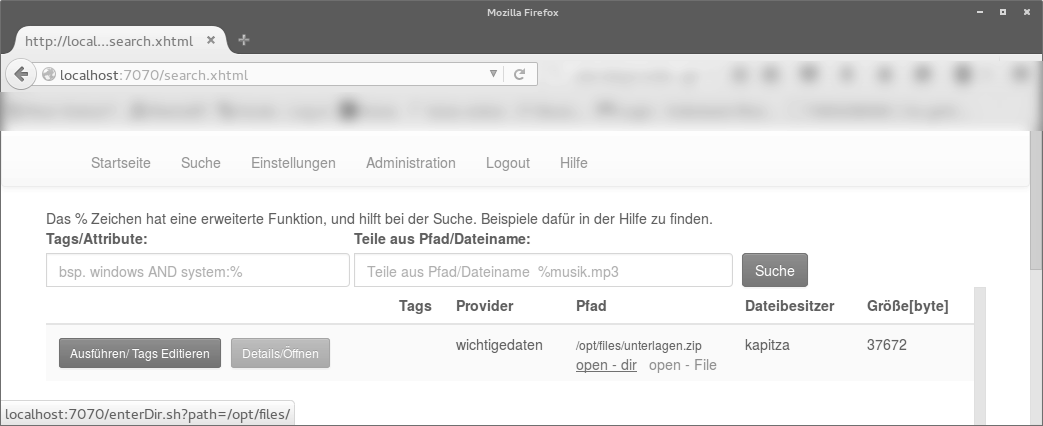
\includegraphics[width=\textwidth]{Masterarbeit_Bilder/original_data_example.png}
    \caption{Ursprüngliche Ausgabe ohne Konfiguration, keine mögliche Nutzung im System, da ,,/opt/files'' nicht existiert.}
    \label{fig:www-orig}
\end{figure}  
\begin{figure}[htbp] 
    \centering
    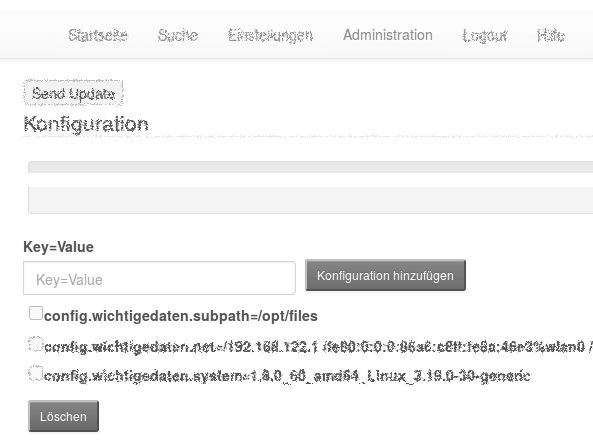
\includegraphics[width=0.8\textwidth]{Masterarbeit_Bilder/admin_remove_sub_cfg.png}
    \caption{Subpath Angabe beim Administrator und löschen von ,,/opt/files'' aus allen Ergebnissen des ,,provider''.}
    \label{fig:www-subpath}
\end{figure}  

\begin{figure}[htbp] 
    \centering
    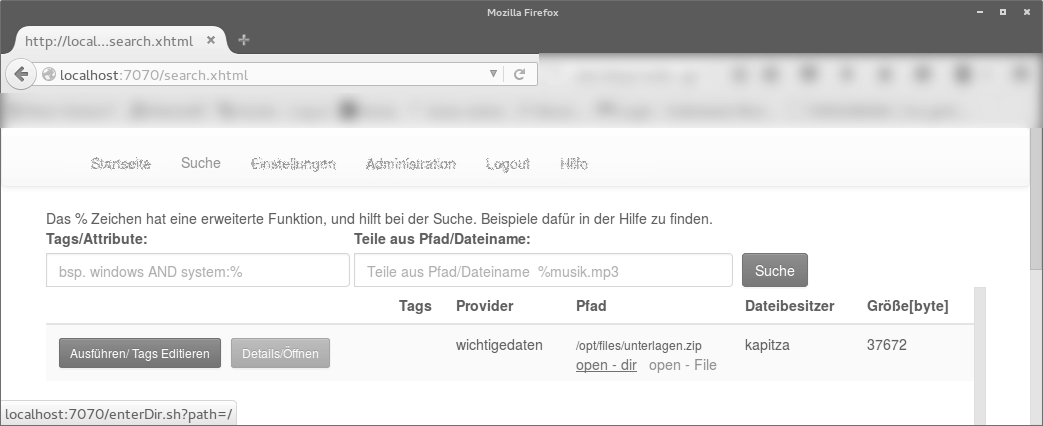
\includegraphics[width=\textwidth]{Masterarbeit_Bilder/admin_remove_sub.png}
    \caption{Ergebnis der ,,subpath'' Angabe beim Administrator nach einer neuen Suche.}
    \label{fig:www-subpath_0}
\end{figure}  
\begin{figure}[htbp] 
    \centering
    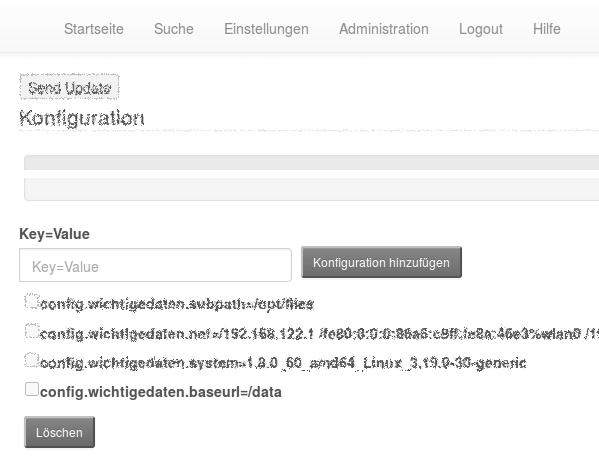
\includegraphics[width=0.8\textwidth]{Masterarbeit_Bilder/admin_change_mount.png}
    \caption{Baseurl Angabe beim Administrator und setzen des PREFIX ,,/data'' auf alle Ergebnisse des ,,provider''.}
    \label{fig:www-subpath2}
\end{figure}  

\begin{figure}[htbp] 
    \centering
    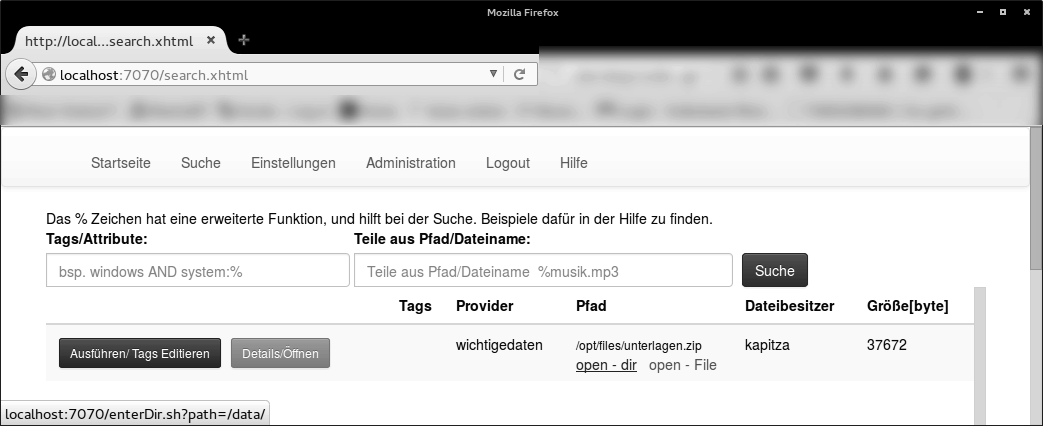
\includegraphics[width=\textwidth]{Masterarbeit_Bilder/open_mount_dir_0.png}
    \caption{Ergebnis der Angaben des Administrator nach einer neuen Suche.}
    \label{fig:www-erg}
\end{figure}  


\begin{figure}[htbp] 
    \centering
    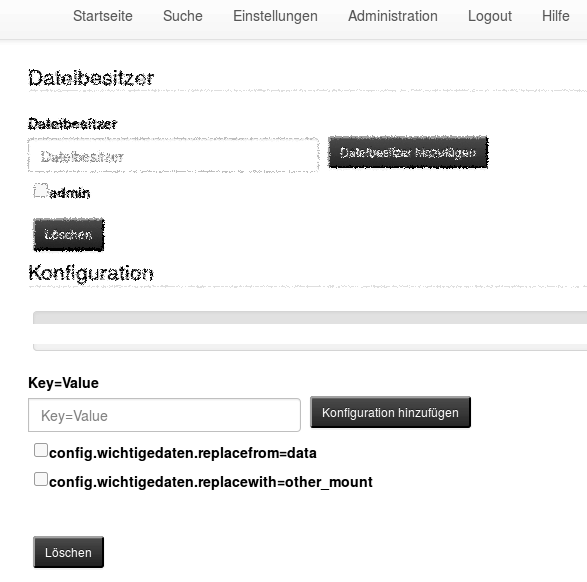
\includegraphics[width=0.8\textwidth]{Masterarbeit_Bilder/user_rewrite_other_mount.png}
    \caption{Neuschreiben der Angaben des Administrator, als Anwender. Der Pfad ,,data'' wird durch ,,other\_mount'' ersetzt. Das System erwartet einen ,,regulären Ausdruck''. }
    \label{fig:www-subpath3}
\end{figure}  

\begin{figure}[htbp] 
    \centering
    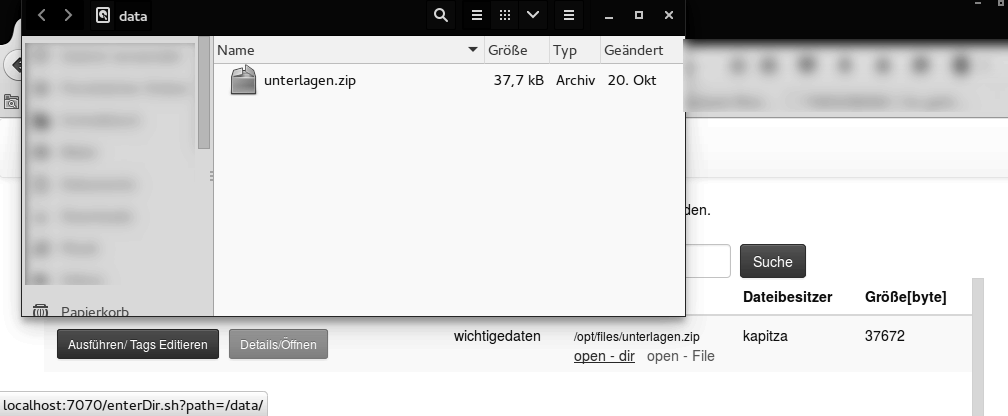
\includegraphics[width=\textwidth]{Masterarbeit_Bilder/open_mount_dir.png}
    \caption{Ergebnis der Angaben des Anwenders, durch Neuschreiben nach einer neuen Suche. Hier ist nach Klicken auf ,,open - dir'' der Dateibrowser ,,nautilus'' im richtigen Ordner geöffnet worden.}
    \label{fig:www-erg2}
\end{figure}  




Da bei den meisten Netzwerken durch den Administrator die Laufwerke festgelegt werden, sollte der durch ihn vorgegebene Standardpfad unter ,,config.{PROVIDER}.baseurl'' für die meisten Anwender ausreichen. Welches Protokoll der Eintrag dabei nutzt, ist dem Administrator überlassen und könnte genauso ,,ftp://SERVER\_FQDN/wichtig'' lauten.
% das gleiche angeben wie OBEN
Die Abbildungen \ref{fig:www-subpath} und \ref{fig:www-subpath2} zeigen die Konfiguration für Linux mit ,,sshfs'' und das daraus resultierende Ergebnis in Abbildung \ref{fig:www-erg}.

Das direkte Arbeiten auf einer Datei bleibt weiterhin dem Betriebssystem überlassen. Die Anwendung hilft durch die generierten Scripte nur beim Navigieren zu den Dateien. Durch einfaches Klicken auf ,,open - dir'' öffnet sich der Dateibrowser an entsprechender Stelle. Es bleibt jedoch die Problematik offen, eine Datei vorab auszuwählen. Sind die Dateisammlungen groß, muss der Anwender im Fenster nach dem richtigen Dateinamen suchen. Geht es lediglich um ein ,,Öffnen'' der Datei mit einer Standardanwendung, sollte ein ,,open - file'' ausreichen, um durch das generierte Script die Datei mit der hinterlegten Anwendung zu öffnen.
%% ralf?
Weiterführende Integration in den Desktop und ein Vermeiden von Scripten, erfordern ein Addon im Browser oder eine separate Anwendung auf dem Endgerät. Es ist in HTML nicht möglich, bestimmte Standardanwendungen in der Weboberfläche zu verwenden. Dies wäre jedoch für eine Dateiverwaltung hilfreich.

 
\subsubsection{Synchronisation der Daten}
Dieses Szenario wird von dieser Anwendung kaum unterstützt. Es ist einzig die Möglichkeit gegeben zwischen zwei Peers Dateien auszutauschen, indem der interne ,,publish''-Befehl freigegeben wird. Jedoch erfordert es immer noch das Eingreifen eines Anwender, der die Datei erst noch veröffentlichen muss, was hinsichtlich der rechtlichen Lage wünschenswert ist. Durch Eintippen von ,,publish'', wie in Abbildung \ref{fig:www-cmd-pub} zu sehen, wird die entsprechende Datei dann allen angemeldeten ,,provider'' übertragen.

\begin{figure}[htbp] 
    \centering
    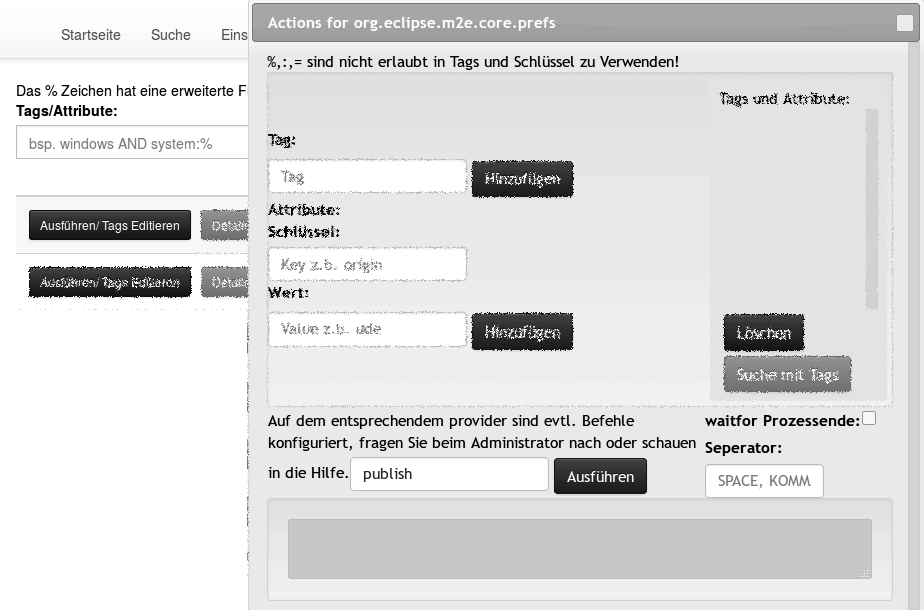
\includegraphics[width=\textwidth]{Masterarbeit_Bilder/www_cmd_publish.png}
    \caption{ ,,publish'' Befehl auf dem ,,provider'' auslösen. Der Empfänger meldet sich direkt nach entsprechender Nachricht des  ,,provider'' um einen Dateiaustausch zu starten. Beim Melden überträgt der Empfänger seine Verbindungsinformationen.}
    \label{fig:www-cmd-pub}
\end{figure}  

\bigskip

Hier bedarf es noch einiges an Arbeitszeit, um einen einfachen Synchronisationsmechanismus zu erstellen, wie er von Diensten wie ,,Dropbox'' oder ,,Google Drive'' bekannt ist.

 
\chapter{Abschlussbetrachtung}
 
\chapmd{Projektmanagementkurs Universität Duisburg-Essen}{,,Ich will, dass Sie so gut werden, dass es mich meinen Job kostet.''}


Nachfolgend wird ein Testaufbau beschreiben und auftretende Probleme diskutiert. Der Versuchsaufbau bezieht sich nachfolgend auf Linux Systeme und umfasst einen Client, der via Webbrowser die ,,www'' Anwendung bedient und eine Weboberfläche für E-Mail verwendet.
Die Testumgebung besteht aus zwei Servern und einem Client. Der zweite Server wird extern verwaltet und ist lediglich für E-Mails zuständig, die vom Benachrichtigungssystem benötigt werden. Das Einrichten und Verwalten eines Mailserver wird hier nicht berücksichtigt. Es wird davon ausgegangen, dass eine gültige E-Mail-Adresse mit passendem Benutzer-Account existiert, um dem Peer ,,database'' den nötigen Zugriff zu ermöglichen. Eine weitere Annahme ist, dass der Mailserver ohne Probleme durch die Firewall erreicht werden kann.

Einen Datenserver mit Netzwerknamen ,,fileserver'', dessen Daten unter ,,/opt/files'' liegen, wird durch ,,sshfs'' am Client unter dem Pfad ,,/data'' gemountet.

Der Datenserver und Client befinden sich im gleichen Netzwerk und sind nicht durch eine Firewall explizit gesichert. Auf dem Datenserver ist Java 8 installiert und es werden als Dienste nur ,,ssh'' sowie die in der Arbeit beschriebenen Projekte ,,database'', ,,www'', ,,master'' und ,,provider'' ausgeführt. Da der ,,master'' eingebettet bereits ,,database'' und ,,www'' startet, muss im verwendeten Speicherort nur noch der ,,provider'' gestartet werden, um die Analyse für  dort liegende Dateien zu starten und zu überwachen.

Das Starten erfolgt mit einfachen Befehlen in der Konsole. Meist reicht ein Doppelklick aus, um mit Standardwerten die Anwendung auszuführen. 

\bigskip

Starten des ,,master'' mit: 
\begin{quote}
    cd /PATH\_TO\_DOWNLOAD\_DIR/ \\
    unzip master-VERSION.zip \\
    cd master \\
    java -jar master-VERSION.jar 
\end{quote}

Die Konfiguration wird aus der Datei ,,server.properties'' gelesen und beinhaltet das Geheimnis, die Konfiguration für E-Mail und Webanwendung.

\bigskip

Der ,,provider'' wird mit:
\begin{quote}
    
    cd /PATH\_TO\_DOWNLOAD\_DIR/ \\
    unzip provider-VERSION.zip \\
    cd provider \\
    Allgemein: java -jar provider-VERSION.jar (provider.properties WATCH\_DIRS ...)\\
    Beispiel: java -jar provider-VERSION.jar provider.properties /opt/files
\end{quote}

gestartet. Es ist beim Start möglich, die Konfiguration und die Pfade der Ordnerüberwachung mitzugeben. Dazu muss die Konfigurationsdatei für die Kommunikation sowie eine Liste von Ordner angegeben werden. Ist kein Parameter gegeben, ist der Standard ,,provider.properties'' und als zu beobachtender Ordner der ,,aktuelle'' Pfad.


Dadurch sind auf dem Server alle Dienste bereitgestellt.
Auf dem Client wird das Laufwerk mit ,,sshfs user@fileserver:/opt/files /data'' eingebunden.

Jedoch liefert ein Zugriff auf die Weboberfläche nicht das gewünschte Ergebnis (Abbildung \ref{fig:www-orig}), da hier hinter der URL noch der falsche Pfad vom Server übertragen wird. Durch eine administrative Einstellung wird nun der Pfad geändert. In Abbildungen \ref{fig:www-subpath} und \ref{fig:www-subpath2} als Administrator global oder durch den Anwender vgl. Abbildung \ref{fig:www-subpath3}. Das Ergebnis ist in beiden Fällen gleich und in Abbildung \ref{fig:www-erg} zu sehen.



\section{Probleme und Schwächen}

Bei der Anwendung sind einige Funktionen wie die Integration in den Desktop nur über Umwege realisierbar gewesen. Der Weg über Scripte ist vergleichbar mit dem Satz:
,,Einen Schraubendreher nutzen, um einen Nagel zu versenken'' \cite{cederholm2009web}. Deswegen ist festzuhalten, dass eine solche Anwendung nicht ohne Addons im Webbrowser vernünftig umsetzbar ist. Da jedoch zu viele verschiedene Webbrowser existieren, ist die Realisierung durch eine separate Client-Anwendung sinnvoller.

In dem erzeugten \acrshort{p2p}-Netzwerk wird idealerweise davon ausgegangen, dass sich die Peers untereinander vertrauen und sich alle Peers regelkonform verhalten.
Das ist jedoch selten der Fall.

Da in den meisten Dateisystemen Sonderzeichen als Dateinamen verboten sind, wird hier nicht beachtet, dass ein Script als Dateinamen kodiert auf einem Client ausgeführt werden könnte \cite{winforbit}. Sollten Dateien mit einem Namen wie \verb|<script>alert('bad javascript')</script>| existieren, dann könnte an einigen Stellen im Code von ,,www'' dieses Script im Webbrowser ausgeführt werden. Da diese Fälle nur künstlich erzeugt werden können, blieb dieses Problem unbeachtet.

Auch das Herausfinden der Existenz einer Datei ist auf einem Peer nicht effizient gelöst, da für jede Datei im Betriebssystem nachgefragt werden muss.
Dabei wird jedes mal von der Festplatte gelesen.
Schneller feststellen, ob eine Datei nicht existiert, könnte bei den Peers durch ,,Bloom Filter'' realisiert werden. Dies würde die Festplatte nicht unnötig  zum Anlaufen bringen, um festzustellen, dass die Datei nicht vorhanden ist. Da für ein definitives Ja dennoch auf die Platte geschaut werden muss, sollte ein Cache in zweiter Ebene und erst als letzte Möglichkeit der Plattenzugriff erfolgen \cite{bejeck2013getting}.  

Fehlerhafte Programme, die beim Ändern einer Datei diese löschen und komplett neu schreiben, können den ,,provider'' behindern und dafür sorgen, dass die Prüfsumme der Datei neu berechnet wird. Bei den angenommenen Dateigrößen ist das nicht wünschenswert, der Fehler lässt sich aber nicht durch das Programm selbst erkennen. Programme, die das Änderungsdatum aktualisieren gehören ebenso dazu, da die Prüfsumme mit dem Änderungsdatum zusammenhängen.

Probleme beim Speichern von Prüfsummen haben im Test gezeigt, dass stillschweigend die alten Attribute mit den neuen überschrieben werden, wenn der Speicherplatz für diese nicht ausreicht. Daher wurde die Limitierung auf wenige Variablen und Attribute in den Dateien gemacht. Gerade Linux ist anfällig für dieses Verhalten.
Ein Ansatz mit beschreibenden Dateien im separaten oder gleichen Ordner ist genauso schwer zu verwalten wie eine gleichnamige versteckte Datei, da hier Fehler durch Umbenennen, Verschieben und Kopieren die entsprechende andere Datei nicht beachtet. Einen ,,Watch Service'' dafür zu implementieren, wäre umständlich und könnte Datenbestände nicht zuverlässig zusammenführen.

Das Projekt ,,bridge'' ist als mögliches Konzept zu sehen, um eine übersichtlichere Netzwerkstruktur und bessere administrative Verteilung zu ermöglichen. Dabei hat es jedoch noch Problemen bei der Zyklenerkennung und Verwaltung doppelter Nachrichten. Ein \acrshort{ttl} ist zwar prinzipiell eine Möglichkeit an das Problem heranzutreten, beschränkt aber das Skalieren der Systeme (vgl. ,,Query flooding'').

Bei der Implementierung wurde nicht RAM-sparend gearbeitet, da durch die Verwendung von Hash-Tabellen eine deutlich bessere Geschwindigkeit gegenüber einfachen Listen erzielt wurde. Die heutigen Computer können der Anwendung die mindestens 512 MB Speicher zusichern welche mit entsprechenden Java Optionen im System gesetzt werden.

Auch wenn die Anwendung portabel und betriebssystemunabhängig ist, sind die gelieferten Dateipfade durch Kodierungen und Konventionen an die Plattform gebunden auf der die Anwendung ausgeführt wird. Es bedarf daher immer dem Eingreifen des Anwender, um durch ,,reguläre Ausdrücke'' den korrekten Pfad für das Endgerät zu erzeugen.

Durch die verwendeten Bibliotheken sind einige Probleme entstanden, die im Rahmen der Arbeit nicht lösbar sind. Darunter ist eine ,,OutOfMemory-Exception'', die vom \acrshort{jms} erzeugt wird, weil die verwendete Pufferung nicht freigegeben wird. Das Auftreten scheint jedoch mit ,,Hibernate-to-Ram'' des Laptop zusammenzuhängen. 

Da Java 8 noch neu ist, kommen viele Bibliotheken nicht mit der neuen API klar, so dass WELD als CDI-Umgebung und \acrshort{jpa} nur mit Java 7 Code ausgeführt werden können.
Eine Eigenart beim \acrshort{orm} durch das ,,ManyToMany'' und den Gebrauch von Join-Tabellen  ermöglicht kein einfaches Löschen ohne weiteres Anlegen von Java-Klassen. Es wurde hier auf eine ,,Embedded Collection'' umgestellt, jedoch ist in den entsprechenden Tabellen nicht die Prüfsumme der Fremdschlüssel, sondern die ID der Datei. So musste das Problem der Zuordnungen der Schlagworte in der Anwendung realisiert werden.
,,Normalisierte'' Tabellen sind daher nicht verwendbar, da die Anwendung dadurch komplexer wird.

Das \acrshort{jpa}  erlaubt ,,lazy-loading'', welches in dieser Anwendung explizit  abgestellt wurde.
Der Grund dafür ist, dass bei einer Datenübertragung im \acrshort{jms}  kein Nachladen, der fehlenden Informationen, erfolgte. Ob dies mit Java 8 zusammen hängt oder aufgrund des eingebetteten Modus wurde nicht evaluiert. Als Lösung wurde der ,,EAGER'' Modus bei den Schlagworten und Hash-Listen verwendet.

Einschränkungen des eingebetteten Modus sind zudem mangelnde Unterstützung von Validierungen durch Notationen im JSF und \acrshort{cdi} Umfeld.
Hier scheint das Problem die verwendete Version des Anwendungsserver zu sein. Im eingebetteten Modus werden von diesem nicht alle API geladen und konfiguriert. Kurz vor Ende der Arbeit ist ein Update angekündigt worden, welches nicht getestet wurde.


Windows als ,,provider'' hat durch installierte Firewall und Virenscanner im Test gezeigt, dass Fehler nicht angezeigt werden. Die Software war nicht ohne administratives Handeln in der Lage, einen Port zur Kommunikation zu öffnen. Der Kommunikationsport muss neben dem festlegen in der Konfigurationsdatei auf dem Betriebssystem und ggf. im Virenscanner entsprechend eingestellt werden. Das bekannte Benachrichtigungsfenster der Windowsfirewall scheint nicht mehr zu existieren. Die zweite Firewall, meist mit  \acrshort{nat}, muss anschließend immer noch überwunden werden. Unauffälliger ist dabei die höhere CPU-Last, da Windows zu viele Events bei der Dateiüberwachung liefert, welche erst durch den selbst geschriebenen Service reduziert werden.

Beim Erstellen der Weboberfläche ist in heutigen Anwendungen ,,Ajax'' in Verwendung. Jedoch ist bei Verwendung von Formularen, welche durch ein angepasstes Javascript verbessert wurden, ein Fehler in JSF aufgefallen. Informationen zu Lösung finden sich im ,,duke.js''-Javascript. 


\subsection{Mac OS und der Webbrowser}
Nach einigen Tests auf einem Mac OS-Rechner, kann festgestellt werden, dass das Ausführen der Scripte, welches von der ,,www''-Anwendung generiert wird, nicht automatisch zur Ausführung konfiguriert werden kann. Die Sicherheitseinstellungen sind mit normalem Anwenderwissen nicht umzustellen.
Es bleibt nur der ,,Workaround'' (vgl. Abbildung \ref{fig:apple}) durch das Öffnen eines Terminal welcher die gespeicherten Scripte ausführt.
\begin{figure}[htbp] 
    \centering
    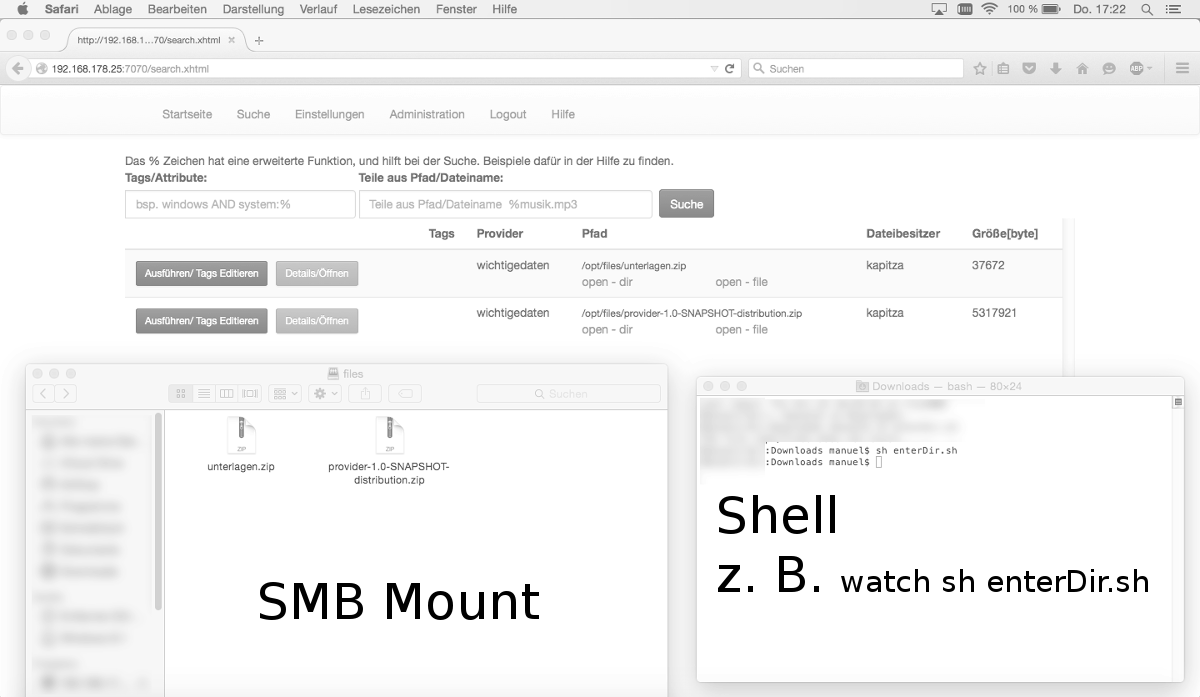
\includegraphics[width=0.8\textwidth]{Masterarbeit_Bilder/appel_terminal.png}
    \caption{Mac OS, Konfigurierter SMB mount ,,files'', der durch das Terminal geöffnet wird. }
    \label{fig:apple}
\end{figure}  

Eine Automatisierungshilfe könnte das Nutzen des ,,watch''-Befehls sein. Dieser kann mit ,,brew'' oder ,,port'' installiert werden. 
Eine Simulationsannäherung wäre durch \verb|while :; do clear; your_command; sleep 2; done| gegeben.
Als Befehl würde die gespeicherte Datei in Downloads ausgeführt werden. Das wäre beispielsweise mit \verb|watch enter.sh| möglich.
Ein automatisches Speichern ist in Safari oder Firefox Einstellbar.


 
 

\section{Zusammenfassung und Ergebnis}
Zum Reflektieren der Anforderungen werden diese der aktuellen Realisierung gegenübergestellt.


\begin{itemize}
	\item Zuordnung einer Person zu den diversen Konten und zu einer Datei als Besitzer/ Verantwortlicher
    
	Diese Aufgabe muss durch den Anwender über eine entsprechende Oberfläche vorgenommen werden. Die Zuordnung als Dateibesitzer kann in den Einstellungen -- wie in Abbildung \ref{fig:app-cfg-datei} zu sehen ist -- gemacht werden. Nötige Informationen  stammen vom ,,provider'' und ausgewählte Daten werden in den ,,database''-Peers gespeichert.
	
	\item Auslesen der Informationen einer Datei unter Beachtung des Dateisystems 
    
	Durch das Java NIO werden das Auslesen und die Überwachung der Änderungen im Dateisystem bereitgestellt.
    Eine Implementierung ist im ,,provider'' realisiert.

    \item Anzeigenanpassung und individuelle Unterstützung je nach verwendeter Plattform 
    
	Das JSF sowie die verwendeten HTML5-Elemente sind Grundlage der Anzeigen und bedürfen keiner Anpassung. Für die Integration wird entsprechend der Plattform ein Script generiert.
    
	\item Übertragung der Dateien zwischen den DMS
    
   Diese wird nicht direkt ersichtlich vom System unterstützt. Eine Freigabe des ,,publish''-Befehl ermöglicht dafür nötige Funktionen. Das manuelle Eingreifen durch den Anwender ist hier zwingend erforderlich.
   
	\item Benachrichtigung über den Vorgang einer Datei
    
	Das System versendet eine E-Mail an den hinterlegten Besitzer der Datei. Sollte keine E-Mail-Adresse bekannt sein, entfällt diese Funktion. Diese Funktion ist in der ,,database'' implementiert.
   
	\item Persistente plattformübergreifende Speicherung von Dateiattributen
    
	Es wird eine Datenbank verwendet, um Attribute plattformunabhängig zu speichern.
    Die einzigen, welche in den ,,erweiterten Attributen'' gespeichert werden, sind die Prüfsumme und deren Erzeugungsdatum. Um konkurrierende Zugriffe zu vermeiden, wird ein drittes Attribut als Sperre verwendet. Der Grund für die begrenzte Speicherung liegt in der schlechten Linux Systemunterstützung.

    Im Dateisystem kann je nach Plattform nachgesehen werden, ob zu einer Datei die Prüfsummen berechnet wurden:
    \begin{itemize}
        \item Windows mit \verb|dir /r|
        \item Linux mit \verb|attr -l|
        \item Mac OS mit \verb|xattr|
    \end{itemize}
    
    und der entsprechenden Datei als Parameter.
    
	\item Verlinken der DMS 
    
    Ein Konzept ist mit der ,,bridge'' beschreiben worden.
    
	\item Erkennung doppelter Dateien
    
    Durch die Oberfläche kann nach Prüfsummen gesucht werden. Eine spezielle Oberfläche, die all doppelten Dateien auflistet, muss noch realisiert werden. Das ,,database''-Projekt bedarf dafür jedoch eine Anpassung, um eine entsprechende nötige Anfrage an die Datenbank zu stellen.
\end{itemize}



\section{Diskussion und Ausblick}
Diese Anwendung unterstützt hinsichtlich der Aufgabenstellung die Suche und eine einfache Dateisynchronisierung.
Wegen der Verwendung von HTTP ist es nicht möglich große Datenmengen zu transportieren, deshalb muss ein weiterer separater Dienst erstellt werden. Eine Möglichkeit wäre, die Realisierung durch eine Implementierung eines SSH-Dienstes, welcher Transfer, Tunnelaufbau und Befehlsausführung realisiert. 

In der Planung wurde beachtet, dass ein Übertragen ähnlicher Dateien berücksichtigt wird, um Verschiebungen zu erkennen. Das erfordert jedoch ein verzögertes Löschen.

Die Nutzung externer Befehle macht das Programm sehr flexibel und Analysen können vom ,,provider'' durch das Nutzen von Apache Tika, wie in der Einleitung erwähnt, verfeinert werden. Diese Bibliothek kann jedoch nicht alle Dateitypen erkennen.

Auch die ,,database'' lässt sich erweitern und durch \href{http://lucene.apache.org/solr/}{ Apache Solr}
besser indizieren.

OSGI ist als Schlagwort im Java-Umfeld immer wieder zu finden. Das macht die Anwendungen jedoch nicht so einfach paketierbar, da eine eingebettete Version selbst bei kleinen Anwendungen anspruchsvoll ist. Auch ist mehr Verwaltung zu Beginn nötig, was das Entwickeln verlangsamt. Der ,,overhead'' bei kleinen Anwendungen ist durch die nötigen Dienste zu groß.

\subsection{Version 2.0}
Wie oben bereits angesprochen, ist ein SSH-Dienst sehr flexibel. Die Integration des Dienstes in die Anwendung würde ein Vermitteln zwischen den Peers durch Tunnel vereinfachen. Die Kommunikation könnte vom \acrshort{jms} auf die Kontrollverbindung des SSH umgestellt werden und würde durch Zertifikate die Sicherheit in der Kommunikation und Authentifizierung bringen. Beim Vermitteln würde das Mitlesen der Daten nicht möglich sein, sofern die betroffenen Peers ihre Fingerprints zuvor ausgetauscht haben.

Dieser Ansatz wird in ,,Version 1.0'' nicht verfolgt, weil die Generierung von Zertifikaten komplex ist und keine einfache Möglichkeit existiert, im Programmcode dies in vorgegebener Zeit zu automatisieren.
Es existieren eine Menge Bibliotheken für SSH, jedoch nur wenige, die einen Server implementiert haben.
SSH besteht aus mehreren kleinen Diensten und die getesteten Bibliotheken wie ,,Apache SSHD'' unterstützen nicht alle Funktionen, um eine Anwendung auf deren Basis zu realisieren.

Die meisten Bibliotheken verbinden sich auf Linux Server, was den Anforderungen, Plattform unabhängig zu sein, widerspricht. Es existieren zwar viele Portierungen des Openssh-Server, jedoch binden gerade unter Linux diese Dienste an das Betriebssystem an und lassen sich nur schwerlich für die Anwendung nutzen, ohne komplexe Konfigurationen zu erstellen.

\subsection{Entwicklung}
Das Projekt wird auf Github:\\
 \verb|https://github.com/JensKapitza/sciserver| \\ 
weiter entwickelt.

Die CD beinhaltet:
\begin{itemize}
    \item \LaTeX - Code, Java Code [keine Bibliotheken die durch Maven installierbar sind], Java Distribution ZIP (,,master''-Peer und ,,provider''-Peer, die das Ausführen der Anwendung ermöglichen)
\end{itemize}



% Anhang
\appendix
\cleardoublepage{}


\printindex
\printglossaries


% Literaturverzeichnis
\backmatter{}

% Sprache für Literaturverzeichnis wählen
%\nocite{de}
%\nocite{en}
%teilweise verändert, aus der Webseite: 
% http://www.is.uni-due.de/lehre/bachelor_und_masterarbeiten/aufbau_einer_abschlussarbeit/
% 
\bibliographystyle{Formatvorlage_IS}
%\bibliographystyle{apalike}
\bibliography{books}



\end{document}